\documentclass[a4paper,11pt]{article}

\usepackage{times}
\usepackage{graphicx}

\hyphenation{Message-Router Text-Query}

\newenvironment{gsc}% Greenstone text bits
{\begin{footnotesize}\begin{tt}}%
{\end{tt}\end{footnotesize}}
 
\newcommand{\gst}[1]{{\footnotesize \tt #1}}

\newcommand{\gsii}{Greenstone2}
\newcommand{\gsiii}{Greenstone3}
\newcommand{\gs}{Greenstone}

\begin{document}

\title{\gsiii\ : A modular digital library.}

% if you work on this manual, add your name here
\author{Katherine Don \\[1ex]
        Department of Computer Science \\
        University of Waikato \\ Hamilton, New Zealand \\ }

\date{}

\maketitle

\newenvironment{bulletedlist}%
{\begin{list}{$\bullet$}{\setlength{\itemsep}{0pt}\setlength{\parsep}{0pt}}}%
{\end{list}}

\noindent
Greenstone Digital Library Version 3 is a complete redesign and
reimplementation of the \gs\  digital library software.  The current
version (\gsii) enjoys considerable success and is being widely used.
\gsiii \  will capitalize on this success, and in addition it will
\begin{bulletedlist}
\item improve flexibility, modularity, and extensibility
\item lower the bar for ``getting into'' the \gs\  code with a view to
   understanding and extending it
\item use XML where possible internally to improve the amount of
   self-documentation
\item make full use of existing XML-related standards and software
\item provide improved internationalization, particularly in terms of sort order,
   information browsing, etc.
\item include new features that facilitate additional ``content management''
   operations
\item operate on a scale ranging from personal desktop to corporate library
\item easily permit the incorporation of text mining operations
\item use Java, to encourage multilinguality, X-compatibility, and to permit
   easier inclusion of existing Java code (such as for text mining).
\end{bulletedlist}
Parts of \gs\  will remain in other languages (e.g. MG, MGPP); JNI (Java
Native Interface) will be used to communicate with these.

A description of the general design and architecture of \gsiii\  is covered by the document {\em The design of Greenstone3: An agent based dynamic digital library} (design-2002.ps, in the docs/manual directory).

This documentation consists of several parts. Section~\ref{sec:install} is for administrators, and covers \gsiii\  installation, how to access the library, and some administration issues. Section~\ref{sec:user} is for users of the software, and looks at using the sample collections, creating new collections, and how to make small customizations to the interface. The remaining sections are aimed towards  the \gs\  developer. Section~\ref{sec:develop-runtime} describes the run-time system, including the structure of the software, and the message format. Section~\ref{sec:new-features} describes how to add new features to \gs, such as how to add new services, new page types, new plugins for different document formats.  Section~\ref{sec:distributed} describes how to make \gs\  run in a distributed fashion, using SOAP as an example communications protocol. Finally, there are several appendices, including how to install \gs\  from CVS, some notes on Tomcat and SOAP, and a comparison of \gsii\  and \gsiii\  format statements.
\newpage
\tableofcontents
\newpage
\section{\gs\  installation and administration}\label{sec:install}

This section covers where to get \gsiii\  from, how to install it and how to run it. The standard method of running \gsiii\  is as a Java servlet. We provide the Tomcat servlet container to run the servlet. Standard web servers may  be able to be configured to provide servlet support, and thereby remove the need to use Tomcat. Please see your web server documentation for this. This documentation assumes that you are using Tomcat. To access \gsiii, Tomcat must be started up, and then it can be accessed via a web browser. 

Ant (Java's XML based build tool) is used for compilation, installation and running Greenstone. The \gst{build.xml} file is the configuration file for the Greenstone project, and \gst{build.properties} contains parameters that can be altered by the user.

\subsection{Get and install \gs\ }\label{sec:getandinstall}

\gsiii\  is available for download from Sourceforge:\\
 \gst{https://sourceforge.net/projects/greenstone3}. There are Windows, Linux, and source releases. The binary releases are self-installing executables: download and run the file to install. A series of prompts will guide you through the installation process. The source release is a gzip'd tar file. Unzip and untar this, check build.properties, then run \gst{'ant install'} to configure and compile the code.

The \gsiii\  library can be launched by running the server program. This is accessible from the Start menu on Windows, or by running the \gst{gs3-server.sh/bat} script in the top level \gst{greenstone3} directory. This program will start up the Tomcat web server and launch a browser.

Alternatively, you can start it up using Ant: run \gst{'ant start'}, which starts up Tomcat, then in a browser go to \gst{http://localhost:8080/greenstone3}\\
(or \gst{http://your-computer-name:your-chosen-port/greenstone3}). \\
This gets you to a welcome page containing links to four servlets: the \gst{test} servlet (this allows you to check that Tomcat is running properly); the standard \gst{library} servlet which serves \gst{localsite} site with the \gst{gs2} interface; the \gst{gs3library} servlet which serves \gst{localsite} using the \gst{default} \gsiii-style interface; and the \gst{gateway} servlet, which serves \gst{gateway} site with the \gst{default} interface. The \gst{gateway} site uses a SOAP connection to communicate with \gst{localsite}, and demonstrates the library working in a distributed fashion. The SOAP connection is not enabled by default - to enable it, run \gst{'ant deploy-localsite'}.

\gsiii\  is also available through CVS (Concurrent Versioning System). This provides the latest development version, and is not guaranteed to be stable. Appendix~\ref{app:cvs} describes how to download and install \gsiii\  from CVS.

\subsection{How the library works}

The standard library program is a Java servlet. We use the Tomcat servlet container to present the servlets over the web. Tomcat takes CGI-style URLs and passes the arguments to the servlet, which processes these and returns a page of HTML. As far as an end-user is concerned, a servlet is a Java version of a CGI program. The interaction is similar: access is via a web browser, using arguments in a URL.

Other types of interfaces can be used, such as Java GUI programs. See Section~\ref{sec:new-interfaces} for details about how to make these.

\subsubsection{Restarting the library}

You can restart Tomcat by clicking 'Restart Server' on the little server program. You should restart the server any time you make changes in the following for those changes to take effect:\\
\begin{bulletedlist}
\begin{gsc}
\item \$GSDL3HOME/WEB-INF/web.xml
\item \$GSDL3SRCHOME/packages/tomcat/conf/server.xml
\end{gsc}
\item any classes or jar files used by the servlets
\end{bulletedlist}


\subsection{Directory structure}

Table~\ref{tab:dirs} shows the file hierarchy for \gsiii.
The first part  shows the common stuff which can be shared between
\gs\  users---the source, libraries etc. The second part shows the file hierarchy for the web directory, which comprises the greenstone3 context for Tomcat, and is accessible via Tomcat. The main directories are for sites and interfaces: there can be several sites and interfaces per installation, and they are described in the following section.

Two environment variables used by \gsiii\ are often mentioned in this manual: \gst{\$GSDL3SRCHOME} and \gst{\$GSDL3HOME}. \gst{\$GSDL3SRCHOME} refers to the top-level \gst{greenstone3} directory, while \gst{\$GSDL3HOME} refers to the \gst{web} directory. The web directory contains everything needed to serve the \gsiii\ library using Tomcat, and doesn't necessarily need to live with the rest of the \gsiii\ source.

\begin{table}
\caption{The \gs\  directory structure}
\label{tab:dirs}
{\footnotesize
\begin{tabular}{l p{8cm}}
\hline
\bf directory & \bf description \\
\hline
greenstone3 
  & The main installation directory---\$GSDL3SRCHOME is set to this directory \\
greenstone3/src 
  & Source code lives here \\
greenstone3/src/java/
  & main \gsiii\  java source code \\
greenstone3/src/packages 
  & Imported source packages from other systems e.g. indexing packages may go here \\
greenstone3/lib
  & Shared library files\\
greenstone3/lib/java
  & Java jar files not needed in the \gsiii\  runtime\\
greenstone3/lib/jni
  & Jar files and shared library files (.so, .jnilib, .dll) needed for JNI components \\
greenstone3/resources 
 & any resources that may be needed\\
greenstone3/resources/soap
 & soap service description files \\
greenstone3/bin
  & executable stuff lives here\\
greenstone3/bin/script
  & some Perl and/or shell scripts\\
greenstone3/packages
  & External packages that may be installed as part of greenstone, e.g. Tomcat \\
greenstone3/docs
  & Documentation\\
greenstone3/gli
  & \gs\ Librarian Interface code \\
greenstone3/gs2build
  & collection building code\\
\hline
greenstone3/web
  & This is where the web site is defined. Any static HTML files can go here. This directory is the root directory used by Tomcat when serving \gsiii. \$GSDL3HOME is set to this directory. \\
greenstone3/web/WEB-INF
  & The web.xml file lives here (servlet configuration information for Tomcat)\\
greenstone3/web/WEB-INF/classes
  & Individual class files needed by the servlet go in here, also properties files for java resource bundles - used to handle all the language specific text. This directory is on the servlet classpath\\
greenstone3/web/WEB-INF/lib
  & jar files needed by the servlets go here \\
greenstone3/web/sites
  & Contains directories for different sites---a site is a set of collections and services served by a single MessageRouter (MR). The MR may have connections (e.g. soap) to other sites\\
greenstone3/web/sites/localsite 
  & An example site - the site configuration file lives here\\
greenstone3/web/sites/localsite/collect 
  & The collections directory \\
greenstone3/web/sites/localsite/images 
  & Site specific images \\
greenstone3/web/sites/localsite/transforms 
  & Site specific transforms \\
greenstone3/web/interfaces
  & Contains directories for different interfaces - an interface is defined by its images and XSLT files \\
greenstone3/web/interfaces/default
  & The default interface\\
greenstone3/web/interfaces/default/images
  & The images for the default interface\\
greenstone3/web/interfaces/default/js
  & The javascript libraries for the default interface\\
greenstone3/web/interfaces/default/style
  & The CSS stylesheets for the default interface\\
greenstone3/web/interfaces/default/transforms
  & The XSLT files for the default interface\\
greenstone3/web/applet 
  & jar files needed by applets can go here \\
\hline
\end{tabular}}
\end{table}


\subsection{Sites and interfaces}\label{sec:sites-and-ints}

Sites and interfaces contain the content and presentation information, respectively, for the digital library.
A site is comprised of a set of collections and possibly some site-wide services. An interface (in this web-based servlet context) is a set of images along with a set of XSLT files used for translating xml output from the library into an appropriate form---HTML in general.

One \gsiii\  installation can have many sites and interfaces, and these can be paired in different combinations.  One instantiation of a servlet uses one site and one interface, so every specified pairing results in a new servlet instance.  For example, a single site might be served with two different interfaces. This provides different modes of access to the same content. e.g. HTML vs WML, or perhaps providing a completely different look and feel for different audiences. Alternatively, a standard interface may be used with many different sites---providing a consistent mode of access to a lot of different content.

Collections live in the \gst{collect} directory of a site. Any collections that are found in this directory when the servlet is initialized will be loaded up. Public collections will appear on the library home page, while private collections will be hidden. These can still be accessed by typing in cgi arguments. Collections require valid configuration files, but apart from this, nothing needs to be done to the site to use new collections. Collections added while Tomcat is running will not be noticed automatically. Either the server needs to be restarted, or a configuration request may be sent to the library, triggering a (re)load of the collection (this is described in Section~\ref{sec:runtime-config}).

There are two  sites that come with the distribution: \gst{localsite}, and \gst{gateway}. \gst{localsite} has several demo  collections, while \gst{gateway} has none. \gst{gateway} specifies that a SOAP connection should be made to \gst{localsite}. Getting this to work involves setting up a soap server for localsite: see Section~\ref{sec:distributed} for details. 
There are also two interfaces provided in the distribution: \gst{default} and \gst{gs2}. The default interface is a generic \gsiii\ interface, while the \gst{gs2} interface aims to look like the old \gsii\ interface.

Each site and interface has a configuration file which specifies parameters for the site or interface---these are described in Section~\ref{sec:config}.

\subsection{Configuring Tomcat}\label{sec:tomcat-config}

The file \gst{\$GSDL3HOME/WEB-INF/web.xml} contains the configuration information for Tomcat. It tells Tomcat what servlets to load, what initial parameters to pass them, and what web names map to the servlets.
There are four servlets specified in web.xml (these correspond to the four servlet links in the welcome page for \gsiii): one is a test servlet that just prints ``hello greenstone'' to a web page. This is useful if you are having trouble getting Tomcat set up. The other three are the \gs\  library servlets described in Section~\ref{sec:getandinstall}, \gst{library}, \gst{gs3library} and \gst{gateway}. Each servlet must specify which site and which interface to use. Having multiple servlets provides a way of serving different sites, or the same site with a different style of presentation. \gst{site\_name} and \gst{interface\_name} are just two examples of initialization parameters used by the library servlets. The full list is shown in Table~\ref{tab:serv-init}. 

For more details about Tomcat see Appendix~\ref{app:tomcat}.

\begin{table}
\caption{\gs\  servlet initialization parameters}
\label{tab:serv-init}
{\footnotesize
\begin{tabular}{lp{3.5cm}p{6cm}}
\hline
\bf name & \bf sample value & \bf description \\
\hline
library\_name & library & the web name of the servlet \\
interface\_name & default & the name of the interface to use\\
site\_name & localsite & the name of the local site to use (use either site\_name or the three remote\_site parameters)\\
remote\_site\_name & org.greenstone.site1 & the name of a remote site (can be anything??) \\
remote\_site\_type & soap & the type of server running on the site \\
remote\_site\_address & http://www.greenstone.org/ greenstone3/services/ localsite & The address of the server \\
default\_lang & en & the default language for the interface\\
receptionist\_class & MyReceptionist & (optional) specifies an alternative Receptionist to use (default is DefaultReceptionist)\\
messagerouter\_class & NewMessageRouter & (optional) specifies an alternative MessageRouter to use (default is MessageRouter)\\
params\_class & GS2Params & (optional) specifies an alternative GSParams class to use \\
\hline
\end{tabular}}
\end{table}

\subsection{Configuring a \gs\ library}\label{sec:config}

Initial \gsiii\  system configuration is determined by a set of XML configuration files. Each site has a configuration file that binds parameters for the site, \gst{siteConfig.xml}. Each interface has a configuration file, \gst{interfaceConfig.xml}, that specifies parameters for the interface. Collections also have several configuration files; these are discussed in Section~\ref{sec:collconfig}. 
The configuration files are read in when the system is initialized, and their contents are cached in memory. This means that changes made to these files once the system is running will not take immediate effect. Tomcat needs to be restarted for changes to the interface configuration file to take effect. However, changes to the site configuration file can be incorporated sending a system command to the library.  There are a series of system commands that can be sent to the library to induce reconfiguration of different modules, including reloading the whole site. This removes the need to restart the system to reflect these changes. These commands are described in Section~\ref{sec:runtime-config}.

\subsubsection{Site configuration file}\label{sec:siteconfig}

The file \gst{siteConfig.xml} specifies the URI for the site (\gst{localSiteName}), the HTTP address for site resources (\gst{httpAddress}), any \gst{ServiceClusters} that the site provides (for example, collection building), any \gst{ServiceRacks} that do not belong to a cluster or collection, and a list of
known external sites to connect to.  Collections are not specified in the site
configuration file, but are determined by the contents of the site's
collect directory.

The HTTP address is used for retrieving resources from a site outside the XML protocol. Because a site is HTTP accessible through Tomcat, any files (e.g. images) belonging to that site or to its collections can be specified in the HTML of a page by a URL. This avoids having to retrieve these files from a remote site via the XML protocol\footnote{Currently, sites live inside the Tomcat greenstone3 root context, and therefore all their content is accessible over HTTP via the Tomcat address. We need to see if parts can be restricted. Also, if we use a different protocol, then resources from remote sites may need to come through the XML. Also, if we are running locally without using Tomcat, we may want to get them via file:// rather than http://.}.
 
Figure~\ref{fig:siteconfig} shows two example site configuration files. The first example is for a rudimentary site with no site-wide services,
which does not connect to any external sites. The second example is for a site with one site-wide service cluster - a collection building cluster.  It also connects to the first site using SOAP.
These two sites happen to be running on the same machine, which is why they can use \gst{localhost} in the address. For site \gst{gsdl1} to talk to site \gst{localsite}, a SOAP server must be run for \gst{localsite}. The address of the SOAP server, in this case, is \gst{http://localhost:8080/greenstone3/services/localsite}.


\begin{figure}
\begin{gsc}\begin{verbatim}
<siteConfig>
  <localSiteName value="org.greenstone.localsite"/>
  <httpAddress value="http://localhost:8080/greenstone3/sites/localsite"/>
  <serviceClusterList/>
  <serviceRackList/>
  <siteList/>
</siteConfig>
\end{verbatim}\end{gsc}

\begin{gsc}\begin{verbatim}
<siteConfig>
  <localSiteName value="org.greenstone.gsdl1"/>
  <httpAddress value="http://localhost:8080/greenstone3/sites/gsdl1"/>
  <serviceClusterList>	
    <serviceCluster name="build">
      <metadataList>
        <metadata name="Title">Collection builder</metadata>
        <metadata name="Description">Builds collections in a 
           gsdl2-style manner</metadata>
      </metadataList>
      <serviceRackList>
        <serviceRack name="GS2Construct"/>
      </serviceRackList>
    </serviceCluster>
  </serviceClusterList>
  <siteList>
    <site name="org.greenstone.localsite"
      address="http://localhost:8080/greenstone3/services/localsite"
      type="soap"/>
  </siteList>
</siteConfig>
\end{verbatim}\end{gsc}
\caption{Two sample site configuration files}
\label{fig:siteconfig}
\end{figure}

Another element that can appear in a site configuration file is \gst{replaceList}. This must have an \gst{id} attribute, and may contain one or more \gst{replace} elements. Replace elements are discussed in Section \ref{sec:collconfig}. The list found in a \gst{siteConfig.xml} file can be applied to any collection by adding a \gst{replaceListRef} element (with the appropriate \gst{id} attribute) to its \gst{collectionConfig.xml} file.

\subsubsection{Interface configuration file}\label{sec:interfaceconfig}

The interface configuration file \gst{interfaceConfig.xml} lists all the actions that the interface knows about at the start (other ones can be loaded dynamically). Actions create the web pages for the library: there is generally one Action per type of page. For example, a query action produces the pages for searching, while a document action displays the documents. The configuration file specifies what short name each action maps to (this is used in library URLs for the a (action) parameter) e.g. QueryAction should use \gst{a=q}. If the interface uses XSLT, it specifies what XSLT file should be used for each action and possibly each subaction. This makes it easy for developers to implement and use different actions and/or XSLT files without recompilation. The server must be restarted, however.

It also lists all the languages that the interface text files have been translated into. These have a \gst{name} attribute, which is the ISO code for the language, and a \gst{displayElement} which gives the language name in that language (note that this file should be encoded in UTF-8). This language list is used on the Preferences page to allow the user to change the interface language. Details on how to add a new language to a \gsiii\  library are shown in Section~\ref{sec:interface-language}.

An \gst{optionList} element can be used to disable or enable some optional functionality for the interface. Currently there are three options that can be enabled:

\begin{tabular}{lp{7cm}}
highlightQueryTerms & Whether search term highlighting is available or not\\
berryBaskets & Whether berry basket functionality is available or not\\
displayAnnotationService & Whether any annotation services (specified in the site config file) should be displayed with a document or not. \\
\end{tabular}

An interface may be based on an existing one, for example, the gs2 interface is based on the default interface. This means that it will use any images or templates from the base one unless overridden in the current one. The \gst{baseInterface} attribute of the \gst{<interfaceConfig>} element is used to specify the base interface.
 
\begin{figure}
\begin{gsc}\begin{verbatim}
<interfaceConfig>
  <actionList>
    <action name='p' class='PageAction'>
      <subaction name='home' xslt='home.xsl'/>
      <subaction name='about' xslt='about.xsl'/>
      <subaction name='help' xslt='help.xsl'/>
      <subaction name='pref' xslt='pref.xsl'/>
      <subaction name='nav' xslt='nav.xsl'/><!-- used for the 
            collection header frame -->
      <subaction name="html" xslt="html.xsl"/> <!-- used to put an 
            external page into a frame with a collection header-->
    </action>
    <action name='q' class='QueryAction' xslt='basicquery.xsl'/>
    <action name='b' class='GS2BrowseAction' xslt='classifier.xsl'/>
    <action name='a' class='AppletAction' xslt='applet.xsl'/>
    <action name='d' class='DocumentAction' xslt='document.xsl'/>
    <action name='xd' class='XMLDocumentAction'>
      <subaction name='toc' xslt='document-toc.xsl'/>
      <subaction name='text' xslt='document-content.xsl'/>
    </action>
    <action name='pr' class='ProcessAction' xslt='process.xsl'/>
    <action name='s' class='SystemAction' xslt='system.xsl'/>
    <action name='g' class='GeneralAction'>
      <subaction name="berry" xslt='berry.xsl'/>
    </action>
  </actionList>
  <languageList>
    <language name="en">
      <displayItem name='name'>English</displayItem>
    </language>
    <language name="fr">
      <displayItem name='name'>Fran�ais</displayItem>
    </language>
    <language name='es'>
      <displayItem name='name'>Espa�ol</displayItem>
    </language>
  </languageList>
  <optionList>
    <option name="highlightQueryTerms" value="true"/>
    <option name="berryBaskets" value="true"/>
  </optionList>
</interfaceConfig>
\end{verbatim}\end{gsc}
\caption{Default interface configuration file}
\label{fig:ifaceconfig}
\end{figure}


\subsection{Run-time re-initialization}\label{sec:runtime-config}

When Tomcat is started up, the site and interface configuration files are read in, and actions/services/collections loaded as necessary. The configuration is then static unless Tomcat is restarted, or re-configuration commands issued. 

There are several commands that can be issued to Tomcat to avoid having to restart the server. These can reload the entire site, or just individual collections. Unfortunately at present there are no commands to reconfigure the interface, so if the interface configuration file has changed, Tomcat must be restarted for those changes to take effect. Similarly, if the Java classes are modified, Tomcat must be restarted then too.

Currently, the runtime configuration commands can only be accessed by typing arguments into the URL; there is no nice web form yet to do this. 

The arguments are entered after the \gst{library?} part of the URL. There are three types of commands: configure, activate, deactivate. These are specified by \gst{a=s\&sa=c}, \gst{a=s\&sa=a}, and \gst{a=s\&sa=d}, respectively (\gst{a} is action, \gst{sa} is subaction). By default, the requests are sent to the MessageRouter, but they can be sent to a collection/cluster by the addition of \gst{sc=xxx}, where \gst{xxx} is the name of the collection or cluster. Table~\ref{tab:run-time config} describes the commands and arguments in a bit more detail.

\begin{table}
\caption{Example run-time configuration arguments.}
\label{tab:run-time config}
{\footnotesize
\begin{tabular}{lp{9cm}}
\hline
\gst{a=s\&sa=c} & reconfigures the whole site. Reads in siteConfig.xml, reloads all the collections. Just part of this can be specified with another argument \gst{ss} (system subset). The valid values are \gst{collectionList}, \gst{siteList}, \gst{serviceList}, \gst{clusterList}. \\
\gst{a=s\&sa=c\&sc=XXX} & reconfigures the XXX collection or cluster. \gst{ss} can also be used here, valid values are \gst{metadataList} and \gst{serviceList}. \\
\gst{a=s\&sa=a} & (re)activate a specific module. Modules are specified using two arguments, \gst{st} (system module type) and \gst{sn} (system module name). Valid types are \gst{collection}, \gst{cluster} \gst{site}.\\
\gst{a=s\&sa=d} & deactivate a module. \gst{st} and \gst{sn} can be used here too. Valid types are \gst{collection}, \gst{cluster}, \gst{site}, \gst{service}. Modules are removed from the current configuration, but will reappear if Tomcat is restarted.\\
\gst{a=s\&sa=d\&sc=XXX} & deactivate a module belonging to the XXX collection or cluster. \gst{st} and \gst{sn} can be used here too. Valid types are \gst{service}. \\
\hline
\end{tabular}}
\end{table}
\newpage
\section{Using \gsiii\ }\label{sec:user}

Once \gsiii\ is installed, the sample collections can be accessed. The installation comes with several example collections, and Section~\ref{sec:usecolls} describes these collections and how to use them. Section~\ref{sec:buildcol} describes how to build new collections.

\subsection{Using a collection}\label{sec:usecolls} 

A collection typically consists of a set of documents, which could be text, HTML, word, PDF, images, bibliographic records etc, along with some access methods, or ``services''. Typical access methods include searching or browsing for document identifiers, and retrieval of content or metadata for those identifiers.
Searching involves entering words or phrases and getting back lists of documents that contain those words. The search terms may be restricted to particular fields of the document. 

Browsing involves navigating pre-defined hierarchies of documents, following links of interest to find documents. The hierarchies may be constructed on different metadata fields, for example, alphabetical lists of Titles, or a hierarchy of Subject classifications. Clicking on a bookshelf icon takes you to a lower level in the hierarchy, while clicking on a book or page icon takes you to a document.

In the standard interface that comes with \gsiii\ \footnote{of course, this is all customizable}, collections in a digital library are presented in the following manner. The 'home' page of the library shows a list of all the public collections in that library. Clicking on a collection link takes you to the home page for the collection, which we call the collection's 'about' page. The standard page banner for a collection looks something like that shown in Figure~\ref{fig:page-banner}.

\begin{figure}[h]
  \centering
  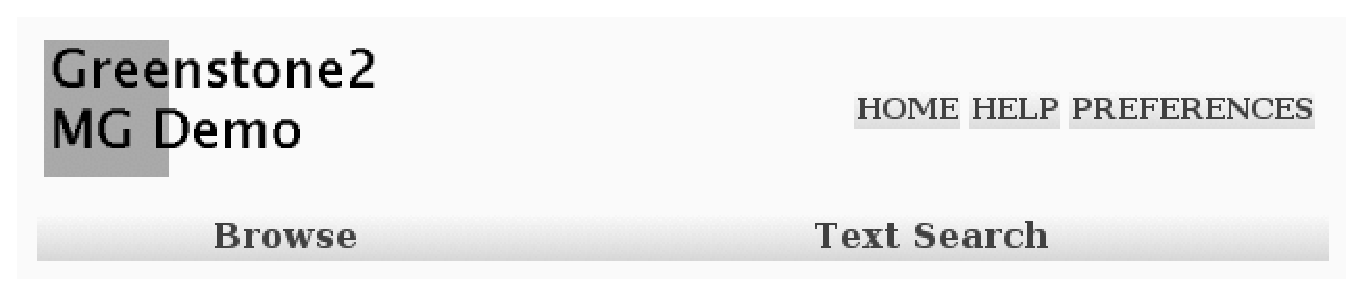
\includegraphics[width=4in]{pagebanner} %5.8
  \caption{A sample collection page banner}
  \label{fig:page-banner}
\end{figure}

The image at the top left is a link to the collection's home page. The top right has buttons to link to the library home page, help and preferences pages. All the available services are arrayed along a navigation bar, along the bottom of the banner. Clicking on a name accesses that service. 

Search type services generally provide a form to fill in, with parameters including what field or granularity to search, and the query itself. Clicking the search button carries out the search, and a list of matching documents will be displayed. Clicking on the icons in the result list takes you to the document itself. 

Once you are looking at a document, clicking the open book icon at the top of the document, underneath the navigation bar, will take you back to the service page that you accessed the document from.

\subsection{Building a collection}\label{sec:buildcol}

There are three ways to get a new collection into \gsiii. The most common way is to use the Greenstone Librarian Interface to create a collection. If you have existing collections in a \gsii\ installation, these can be imported into \gsiii. Thirdly, you can use the Perl command line building scripts directly.

Collections live in the \gst{collect} directory of a site. As described in Section~\ref{sec:sites-and-ints}, there can be several sites per \gsiii\  installation. The collect directory is at \gst{\$GSDL3HOME/sites/site-name/collect}, where site-name is the name of the site you want your new collection to belong to.

The following three sections briefly  describe how to create a collection using GLI, how to import a collection from \gsii, and how to use command line building.  Once a collection has been built (and is located in the collect directory), the library server needs to be notified that there is a new collection. This can be accomplished in two ways\footnote{and eventually there will also probably be automatic polling for new collections}. If you are the library administrator, you can restart Tomcat. The library servlet will then be created afresh, and will discover the new collection when it scans the collect directory for the collection list. Alternatively, an activate collection command can be issued to the servlet, using the arguments \gst{a=s\&sa=a\&st=collection\&sn=collname}, where \gst{collname} should be replaced with the collection name---this tells the library program to (re)load the \gst{collname} collection.

\subsubsection{Using the Librarian Interface}

The Greenstone Librarian Interface (GLI) can be used to create collections. The procedure is the same as for \gsii, but it works in a \gsiii\  context. It can be started under Windows by selecting Greenstone Librarian Interface from the Greenstone 3 Digital Library menu in the Program Files section of the Start menu. On Linux, run \gst{ant gli} from the \gst{greenstone3} directory, or run \gst{./gli4gs3.sh} from the \gst{\$GSDL3SRCHOME/gli} directory.

Currently, the GLI works almost exactly the same as for \gsii\footnote{Eventually the GLI will be modified to use \gsiii\ XML  configuration files.}. Collection configuration is done in a \gsii\ manner. The main difference is that \gsiii\ has different sites and interfaces and servlets, whereas \gsii\ has a single collect directory, and a single runtime cgi program.

The GLI for \gsiii\ has a couple of new configuration parameters: site and servlet. It operates within a single site---you can edit, delete, and create new collections within this site. A servlet is also specified for that site---this is used when previewing a collection. While you are working in one site, you cannot edit collections from another site. However, you can base a collection on one from another site. To change the working site and/or servlet, go to Preferences-$>$Connection in the File menu. By default, the GLI will use site \gst{localsite}, and servlet \gst{library}.

Collection building using the GLI will use the \gsii\ Perl scripts and plugins. At the conclusion of the \gsii\ build process, a conversion script will be run to create the \gsiii\  configuration files. This means that format statements are no longer 'live'---changing these will require changes to the \gsiii\ configuration files. Clicking the Preview Collection button will re-run the configuration file conversion script. If you change anything on the Format panel, you will need to click Preview Collection. Just reloading the collection via a browser will not be enough. 
 
Detailed instructions about using the GLI can be found in Sections 3.1 and 3.2 of the \gsii\  User's Guide (\gst{GS2-User-en.pdf}). This can be found in  your \gsii\ installation, or in the \gst{\$GSDL3SRCHOME/docs/manual} directory if you have installed \gsiii\ from a distribution.


\subsubsection{Importing from \gsii}

Pre-built \gsii\ collections can also be used in \gsiii. The collection folder should be copied to the collect directory of the site it is to appear in (or a symbolic link may be used if possible).
The \gsiii\  run time system requires different configuration files for a collection, so you need to run a conversion script. All this does is create the new \gst{collectionConfig.xml} and \gst{buildConfig.xml} from the old \gst{collect.cfg} and \gst{build.cfg} files. It does not change the collection in any way, so it can still be used by \gsii\  software.

The conversion script is \gst{convert\_coll\_from\_gs2.pl}. To run it, make sure you have run \gst{source setup.bash} (or \gst{setup} in Windows) in the \gst{\$GSDL3SRCHOME/gs2build} directory (as well as running the standard \gst{gs3-setup} command). Then you need to specify the path to the collect directory and the collection name as parameters to the conversion script. For example, 

\begin{gsc}
\begin{verbatim}
convert_coll_from_gs2.pl -collectdir 
   $GSDL3HOME/sites/localsite/collect gs2mgdemo
\end{verbatim}
\end{gsc}
%$
The script attempts to create \gsiii\  format statements from the old \gsii\  ones. The conversion may not always work properly, so if the collection looks a bit strange under \gsiii, you should check the format statements. Format statements are described in Section~\ref{sec:formatstmt}.

Once again, to have the collection recognized by the library servlet, you can either restart Tomcat, or load it dynamically.

\subsubsection{Using command line building}

This is the same procedure as for \gsii\ command line building, with the addition of a final step to create the \gsiii\ configuration files. The basic steps are (for a new collection called testcol):

Linux:

\begin{gsc}
\begin{verbatim}
cd greenstone3
source gs3-setup.sh
cd gs2build
source setup.bash
cd ../
mkcol.pl -collectdir $GSDL3HOME/sites/localsite/collect testcol
put source documents and metadata into 
            $GSDL3HOME/sites/localsite/collect/testcol/import
edit $GSDL3HOME/sites/localsite/collect/testcol/etc/collect.cfg as 
            appropriate
import.pl -collectdir $GSDL3HOME/sites/localsite/collect testcol
buildcol.pl -collectdir $GSDL3HOME/sites/localsite/collect testcol
rename the $GSDL3HOME/sites/localsite/collect/testcol/building 
            directory to index
convert_coll_from_gs2.pl -collectdir $GSDL3HOME/sites/localsite/collect 
            testcol
%$
\end{verbatim}
\end{gsc}

Windows:
\begin{gsc}
\begin{verbatim}
cd greenstone3
gs3-setup
cd gs2build
setup
cd ..
perl -S mkcol.pl -collectdir %GSDL3HOME%\sites\localsite\collect testcol
put source documents and metadata into 
            %GSDL3HOME%\sites\localsite\collect\testcol\import
edit %GSDL3HOME%\sites\localsite\collect\testcol\etc\collect.cfg as 
            appropriate
perl -S import.pl -collectdir %GSDL3HOME%\sites\localsite\collect testcol
perl -S buildcol.pl -collectdir %GSDL3HOME%\sites\localsite\collect testcol
rename the %GSDL3HOME%\sites\localsite\collect\testcol\building directory 
            to index
perl -S convert_coll_from_gs2.pl -collectdir 
            %GSDL3HOME%\sites\localsite\collect testcol
\end{verbatim}
\end{gsc}

Once the build process is complete, Tomcat should be prompted to reload the collection---either by restarting the server, or by sending an activate collection command to the library servlet.

Metadata for documents can be added using \gst{metadata.xml} files.  A \gst{metadata.xml} file has a root element of \gst{<DirectoryMetadata>}.  This encloses a series of \gst{<FileSet>} items.  Neither of these tags has any attributes.  Each \gst{<FileSet>} item includes two parts: firstly, one or more \gst{<FileName>} tags, each of which encloses a regular expression to identify the files which are to be assigned the metadata.  Only files in the same directory as the \gst{metadata.xml} file, or in one of its child directories, will be selected.  The filename tag encloses the regular expression as text, e.g.:

\begin{gsc}\begin{verbatim}
<FileName>example</FileName>
\end{verbatim}\end{gsc}

This would match any file containing the text 'example' in its name.  The second part of the \gst{<FileSet>} item is a \gst{<Description>} item.  The \gst{<Description>} tag has no attributes, but encloses one or more \gst{<Metadata>} tags.  Each \gst{<Metadata>} tag contains one metadata item, i.e. a label to describe the metadata and a corresponding value.  The \gst{<Metadata>} tag has one compulsory attribute: \gst{'name'}.  This attribute gives the metadata label to add to the document.  Each \gst{<Metadata>} tag also has an optional attribute: \gst{'mode'}.  If this attribute is set to \gst{'accumulate'} then the value is added to the document, and any existing values for that metadata item are retained.  If the attribute is set to \gst{'set'} or is omitted, then any existing value of the metadata item will be deleted.

\begin{figure}
\begin{gsc}\begin{verbatim}
<?xml version="1.0" encoding="UTF-8"?>
<!DOCTYPE DirectoryMetadata SYSTEM "http://greenstone.org/dtd/DirectoryMetadata
         /1.0/DirectoryMetadata.dtd">
<DirectoryMetadata>
  <FileSet>
    <FileName>ec160e</FileName>
    <Description>
      <Metadata name="Title">The Courier - No.160 - Nov - Dec 1996 - 
         Dossier Habitat - Country reports: Fiji , Tonga (ec160e)</Metadata>
      <Metadata mode="accumulate" name="Language">English</Metadata>
      <Metadata mode="accumulate" name="Subject">Settlements and housing: 
        general works incl. low- cost housing, planning techniques, surveying, 
        etc.</Metadata>
      <Metadata mode="accumulate" name="Subject">The Courier ACP 1990 - 1996 
        Africa-Caribbean-Pacific - European Union</Metadata>
      <Metadata mode="accumulate" name="Organization">EC Courier</Metadata>
      <Metadata mode="accumulate" name="AZList">T.1</Metadata>
    </Description>
  </FileSet>
  <FileSet>
    <FileName>b22bue</FileName>
    <Description>
      <Metadata name="Title">Butterfly Farming in Papua New Guinea 
        (b22bue)</Metadata>
      <Metadata mode="accumulate" name="Language">English</Metadata>
      <Metadata mode="accumulate" name="Subject">Other animals (micro-
        livestock, little known animals, silkworms, reptiles, frogs, 
        snails, game, etc.)</Metadata>
      <Metadata mode="accumulate" name="Organization">BOSTID</Metadata>
      <Metadata mode="accumulate" name="AZList">T.1</Metadata>
      <Metadata mode="accumulate" name="Keyword">start a butterfly farm
        </Metadata>
    </Description>
  </FileSet>
</DirectoryMetadata>
\end{verbatim}\end{gsc}
\caption{Sample metadata.xml file}
\label{fig:metadatafile}
\end{figure}

Figure~\ref{fig:metadatafile} shows an example metadata.xml file.
Here, only one file pattern is found in each file set.  However, the \gst{Description} tag contains a number of separate metadata items.  Note that the \gst{Title} metadata does not have the \gst{mode=accumulate} attribute.  This means that when this title is assigned to a document, any existing \gst{Title} information will be lost.


\subsection{Collection configuration files}\label{sec:collconfig}

Each collection has two, or possibly three, \gsiii\ configuration files, \\
\gst{collectionConfig.xml}, \gst{buildConfig.xml}, and optionally \gst{collectionInit.xml}, that give metadata, display and other information for the
collection. Currently, \gst{collectionConfig.xml} and \gst{buildConfig.xml} are generated from \gst{collect.cfg} and \gst{build.cfg}. At some stage, the collection building process and the Librarian Interface will be modified to use these files directly. 
\gst{collect.cfg} and/or \gst{collectionConfig.xml} includes user-defined presentation metadata for the collection, such as its name and the {\em About this collection} text; gives formatting information for the collection display; and also gives instructions on how the collection is to be built. \gst{build.cfg} and/or \gst{buildConfig.xml} are produced by the build-time process and include any metadata that can be determined automatically. It also includes configuration information for any ServiceRacks needed by the collection.

All the configuration files should be encoded using UTF-8.

The format of \gst{collect.cfg} and \gst{build.cfg} are not discussed here. Please see the \gsii\ manuals for more information regarding these files.

\subsubsection{collectionInit.xml}

This optional file is only used for non-standard, customized collections. It specifies the class name of the non-standard collection class.  The only syntax so far is the class name:

\begin{gsc}\begin{verbatim}
<collectionInit class="XMLCollection"/>
\end{verbatim}\end{gsc}

Section~\ref{sec:new-coll-types} describes an example collection where this file is used. Depending on the type of collection that this is used for, one or both of the other configuration files may not be needed.

\subsubsection{collectionConfig.xml}

The collection configuration file is where the collection designer (e.g. a librarian) decides what form the collection should take. So far this file only includes the presentation aspects needed by the run-time system. Instructions for collection building have yet to be defined. Presentation aspects include collection metadata such as title and description, display text for indexes, and format statements for search results, classifiers etc. The format of \gst{collectionConfig.xml} is still under consideration. However, Figure~\ref{fig:collconfig} shows the parts of it that have been defined so far. 

Display elements for a collection can be entered in any language---use \gst{lang='en'} attributes to specify which language they are in.

\begin{figure}
\begin{gsc}\begin{verbatim}
<collectionConfig xmlns:gsf="http://www.greenstone.org/greenstone3/
  schema/ConfigFormat" xmlns:xslt="http://www.w3.org/1999/XSL/Transform">
  <metadataList>
    <metadata name="creator">greenstone@cs.waikato.ac.nz</metadata>
    <metadata name="public">true</metadata>
  </metadataList>
  <displayItemList>
    <displayItem name='name' lang='en'>Greenstone3 MG demo collection</displayItem>
    <displayItem name='description' lang='en'>This is a demonstration 
      collection for the Greenstone3 digital library software.</displayItem>
    <displayItem name='icon' lang='en'>gs3mgdemo.gif</displayItem>
    <displayItem name='smallicon' lang='en'>gs3mgdemo_sm.gif</displayItem>
  </displayItemList>
  <search>
    <index name="ste">
      <displayItem name='name' lang="en">chapters</displayItem>
      <displayItem name='name' lang="fr">chapitres</displayItem>
      <displayItem name='name' lang="es">capítulos</displayItem>
    </index>
    [ ... more indexes ...]
    <format>
      <gsf:template match="documentNode"><td valign='top'>
       <gsf:link><gsf:icon/></gsf:link></td><td><gsf:metadata name='Title'/>
      </td></gsf:template>
    </format>
  </search>
  <browse>
    <classifier name="CL1" horizontalAtTop='true'>
      <displayItem name='name' lang='en'>Titles</displayItem>
    </classifier>
    [... more classifiers ...]
    <classifier name="CL4">
      <displayItem name='name' lang='en'>HowTo</displayItem>
      <format>
        <gsf:template match="documentNode">
          <br /><gsf:link><gsf:metadata name='Keyword' />
            </gsf:link></gsf:template>
      </format>
    </classifier>
  </browse>
  <display>
    <format>
      <gsf:option name="coverImages" value="false"/>
      <gsf:option name="documentTOC" value="false"/>
    </format>
  </display>
</collectionConfig>
\end{verbatim}\end{gsc}
\caption{Sample collectionConfig.xml file}
\label{fig:collconfig}
\end{figure}

The \gst{<metadataList>} element specifies some collection metadata, such as creator. The \gst{<displayItemList>} specifies some language dependent information that is used for collection display, such as collection name and short description. These \gst{displayItem} elements can be specified in different languages. 
 
The \gst{<search>} element provides some display and formatting information for the search indexes, while the \gst{<browse>} element concerns classifiers, and   the \gst{<display>} element looks at document display. 

Inside the \gst{<search>} and \gst{<browse>} elements, \gst{<displayItem>} elements are used to provide titles for the indexes or classifiers, while \gst{<format>} elements provide formatting instructions, typically for a document or classifier node in a list of results. Placing the \gst{<format>} instructions at the top level in the \gst{search} or \gst{browse} element will apply the format to all the indexes or classifiers, while placing it inside an individual \gst{index} or \gst{classifier} element will restrict that formatting instruction to that item.

The \gst{<display>} element contains optional formatting information for the display of documents. Templates that can be specified here include \gst{documentHeading} and \gst{DocumentContent}. Other formatting options may also be specified here, such as whether to display a table of contents and/or cover image for the documents.

Format elements are described in Section~\ref{sec:formatstmt}.

An optional \gst{<replaceList>} element can be included at the top level. This contains a list of strings and their replacements. This is particularly useful for \gsii\  collections that use macros. 

The format is like the following:
\begin{gsc}\begin{verbatim}
<replaceList>
<replace scope='text' macro="xxx" text="yyy"/>
<replace scope='metadata' macro="xxx" bundle="yyy" key="zzz"/>
<replace scope='all' macro='xxx' metadata='yyy'/>
</replaceList>
\end{verbatim}\end{gsc}

Scope determines on what text the replacements are carried out: \gst{text}, \gst{metadata}, and \gst{all} (both text and metadata). An empty scope attribute is equivalent to scope=all. Each replace type can be used with all scope values. Replacing uses Java's 'String.replaceAll' functionality, so macro and replacement text are actually regular expressions. The first example is a straight textual replacement. The second example uses dictionary lookups. xxx will be replaced with the (language-dependent) value for key zzz in resource bundle yyy. The third example uses metadata: xxx will be replaced by the value of the yyy metadata for that document.

Appendix~\ref{app:gs2replace} gives some examples that have been used for \gsii\  collections.

\subsubsection{buildConfig.xml}\label{sec:buildconfig}

The file \gst{buildConfig.xml} is produced by the collection building process. Generally it is not necessary to look at this file, but it can be useful in determining what went wrong if the collection doesn't appear quite the way it was planned.

It contains metadata and other information about the collection that can
be determined automatically, such as the number of
documents in the collection.  It also includes a list of \gst{ServiceRack} classes that are
required to provide the services that have been built into the
collection.  The serviceRack names are Java classes that are loaded
dynamically at runtime. Any information inside the serviceRack element is
specific to that service---there is no set format. Figure~\ref{fig:buildconfig} shows an example. This configuration file specifies that the collection should load up 3 ServiceRacks: \gst{GS2Browse}, \gst{GS2MGPPRetrieve} and \gst{GS2MGPPSearch}. The contents of each \gst{<serviceRack>} element are passed to the appropriate ServiceRack objects for configuration. The \gst{collectionConfig.xml} file content is also passed to the ServiceRack objects at configure time---the \gst{format} and \gst{displayItem} information is used directly from the \gst{collectionConfig.xml} file rather than added into \gst{buildConfig.xml} during building. This enables formatting and metadata changes in \gst{collectionConfig.xml} to take effect in the collection without rebuilding being necessary. However, as these files are cached, the collection needs to be reloaded for the changes to appear in the library.


\begin{figure}
\begin{gsc}\begin{verbatim}
<buildConfig>
  <metadataList>
    <metadata name="numDocs">11</metadata>
    <metadata name="buildType">mgpp</metadata>
  </metadataList>
  <serviceRackList>
    <serviceRack name="GS2Browse">
      <indexStem name="gs2mgppdemo"/>
      <classifierList>
        <classifier name="CL1" content="Title"/>
        <classifier name="CL2" content="Subject" />
        <classifier name="CL3" content="Organization" />
        <classifier name="CL4" content="Howto" />
      </classifierList>
    </serviceRack>
    <serviceRack name="GS2MGPPRetrieve">
      <indexStem name="gs2mgppdemo"/>
      <defaultLevel name="Sec" />
    </serviceRack>
    <serviceRack name="GS2MGPPSearch">
      <indexStem name="gs2mgppdemo"/>
      <defaultLevel name="Sec" />
      <levelList>
        <level name="Sec" />
        <level name="Doc" />
      </levelList>
      <fieldList>
        <field shortname="ZZ" name="allfields" />
        <field shortname="TX" name="text" />
        <field shortname="DL" name="dls.Title" />
        <field shortname="DS" name="dls.Subject" />
        <field shortname="DO" name="dls.Organization" />
      </fieldList>
      <searchTypeList>
        <searchType name="form" />
        <searchType name="plain" />
      </searchTypeList>
      <indexOptionList>
        <indexOption name="stemIndexes" value="3"/>
	<indexOption name="maxnumeric" value="4"/>
      </indexOptionList>
      <defaultIndex name="idx" />
      <indexList>
        <index name="idx" />
      </indexList>
    </serviceRack>
  </serviceRackList>
</buildConfig>
\end{verbatim}\end{gsc}
\caption{Sample buildConfig.xml file (gs2mgppdemo collection)}
\label{fig:buildconfig}
\end{figure}

\subsection{Formatting the collection}\label{sec:formatstmt}

\subsubsection{Modifying the ``format'' xslt templates}
Part of collection design involves deciding how the collection should look. \gsiii\  has a default 'look' for a collection, so this is optional. However, the default may not suit the purposes of some collections, so many parts to the look of a collection can be determined by the collection designer.

In standard \gsiii, the library is served to a web browser by a servlet, and the HTML is generated using XSLT. XSLT templates are used to format all the parts of the pages. These templates can be overridden by including them in the \gst{collectionConfig.xml} file. Some commonly overridden templates are those for formatting lists: search results list, classifier browsing hierarchies, and for parts of the document display. 

Real XSLT templates for formatting search results or classifier lists are quite complicated, and not at all easy for a new user to write. For example, the following is a sample template for formatting a classifier list, to show Keyword metadata as a link to the document.
 
\begin{gsc}\begin{verbatim}
<xsl:template match="documentNode" priority="2"
     xmlns:xsl="http://www.w3.org/1999/XSL/Transform">
  <xsl:param name="collName"/>
    <td><a href="{$library_name}?a=d&amp;c={$collName}&amp;
           d={@nodeID}&amp;dt={@docType}"><xsl:value-of 
           select="metadataList/metadata[@name='Keyword']"/></a>
    </td>
</xsl:template>
 \end{verbatim}\end{gsc}
 
To write this, the user would need to know that:
\begin{bulletedlist}
\item the variable \gst{\$library\_name} exists,
\item the collection name is passed in as a parameter called \gst{collName}
\item metadata for a document is found in a \gst{<metadataList>} and that its form is \gst{<metadata name="Keyword">the value</metadata>}
\item the arguments needed for the link to the document are \gst{a, sa, c, d, a, dt}.
\end{bulletedlist}
 
We can use XSLT to transform XML into XSLT. \gsiii\  provides a simplified set of formatting commands, written in XML, which will be transformed into proper XSLT. The user specifies a \gst{<gsf:template>} for what they want to format---these typically match \gst{documentNode} or \gst{classifierNode} (for a node in a classification hierarchy).
 
The template above can be represented as:
 
\begin{gsc}\begin{verbatim}
<gsf:template match='documentNode'>
  <td><gsf:link><gsf:metadata name='Keyword'/></gsf:link></td>
</gsf:template>
\end{verbatim}\end{gsc}

Table~\ref{tab:gsf-format} shows the set of \gst{'gsf'} (Greenstone Format) elements. If you have come from a \gsii\  background, Appendix~\ref{app:gs2format} shows \gsii\  format elements and their equivalents in \gsiii\ .
 
\begin{table}
\caption{Format elements for GSF format language}
\label{tab:gsf-format}
{\footnotesize
\begin{tabular}{p{6.5cm}p{6.5cm}}
\hline
\bf Element       & \bf Description \\
\hline
\gst{<gsf:text/>} & The document's text\\
\hline
\gst{<gsf:link>...</gsf:link>} & The HTML link to the document itself \\
\gst{<gsf:link type='document'>...
</gsf:link>} & Same as above\\
\gst{<gsf:link type='classifier'>...
</gsf:link>} & A link to a classification node (use in classifierNode templates)\\
\gst{<gsf:link type='source'>...
</gsf:link>} & The HTML link to the original file---set for documents that have been converted from e.g. Word, PDF, PS \\
\hline
\gst{<gsf:icon/>}  & An appropriate icon\\
\gst{<gsf:icon type='document'/>} & same as above\\
\gst{<gsf:icon type='classifier'/>} & bookshelf icon for classification nodes\\
\gst{<gsf:icon type='source'/>} & An appropriate icon for the original file e.g. Word, PDF icon\\
\hline
\gst{<gsf:metadata name='Title'/>} & All the values of a metadata element for the current document or section, in this case, Title\\
\gst{<gsf:metadata name='Title' select='select-type' [separator='y' prefix="p" suffix="s" pos='first|last|n']/>} & A more extended selection of metadata values. The select field can be one of those shown in Table~\ref{tab:gsf-select-types}. There are some optional attributes: separator gives a String that will be used to separate the fields (default is ``, ``), prefix and suffix give strings that will be output before and after each field, and pos can be set to return either the first, last or nth value for that metadata at each section.\\
\gst{<gsf:metadata name='Title'> <separator>y</separator> <prefix>p</prefix> <suffix>s</suffix> </gsf:metadata>} & separator, prefix and suffix can all be specified as elements instead of attributes. This format allows for HTML tags to be used. e.g. \gst{<br/>} as a separator. \\
\gst{<gsf:metadata name='Date' format='formatDate'/>} & The value of a metadata element for the current document, formatted in some way. Current formatting options available are listed in Table~\ref{tab:gsf-process-types}. \\
\hline
\gst{<gsf:choose-metadata>
  <gsf:metadata name='metaA'/>
  <gsf:metadata name='metaB'/>
  <gsf:metadata name='metaC'/>
</gsf:choose-metadata>}
 & A choice of metadata. Will select the first existing one. the metadata elements can have the select, separator and pos attributes like normal.\\
\hline
\gst{<gsf:switch preprocess=
'preprocess-type'>
<gsf:metadata name='Title'/> 
<gsf:when test='test-type'
test-value='xxx'>...</gsf:when>
<gsf:when test='test-type' 
test-value='yyy'>...</gsf:when>
<gsf:otherwise>...</gsf:otherwise>
</gsf:switch>} & switch on the value of a particular metadata - the metadata is specified in gsf:metadata, has the same attributes as normal.\\
\hline
\end{tabular}}
\end{table}

The \gst{<gsf:metadata>} elements are used to output metadata values. The simplest case is \gst{<gsf:metadata name='Title'/>}---this outputs all the Title metadata values for the current document or section. Namespaces are important here: if the Title metadata is in the Dublin Core (dc) namespace, then the element should look like \gst{<gsf:metadata name='dc.Title'/>}. There are three other attributes for this element. By default, more than one value for the selected metadata is returned, where multiple exist. The attribute \gst{pos} is used when a particular value for the selected metadata is requested (which can be the first, last or nth value). 
For instance, one document may fall into several classification categories, and therefore may have multiple Subject metadata values. When all are returned, the multiple values are separated by commas by default. The \gst{separator} attribute is used to change the separating string. For example, adding \gst{separator=':~'} to the element will separate all values by a colon and a space. Instead of retrieving all values for a piece of metadata, adding \gst{pos='first'} to the \gst{<gsf:metadata>} element will retrieve the first value.

Sometimes you may want to display metadata values for sections other than the current one. For example, in the mgppdemo collection, in a search list we display the Titles of all the enclosing sections, followed by the Title of the current section, all separated by semi-colons. The display ends up looking something like:
\emph{Farming snails 2; Starting out; Selecting your snails}
where \emph{Selecting your snails} is the Title of the section in the results list, and \emph{Farming snails 2} and \emph{Starting out} are the Titles of the enclosing sections. The \gst{select} attribute is used to display metadata for sections other than the current one. Table~\ref{tab:gsf-select-types} shows the options available for this attribute. The \gst{separator} attribute is used here also, to specify the separating text.

To get the previous metadata, the format statement would have the following in it:

\begin{gsc}
\begin{verbatim}
<gsf:metadata name='Title' select='ancestors' separator='; '/>; 
    <gsf:metadata name='Title'/>
\end{verbatim}
\end{gsc}

\begin{table}
\caption{Select types for metadata format elements}
\label{tab:gsf-select-types}
{\footnotesize
\begin{tabular}{ll}
\hline
\bf Select Type & \bf Description\\
\hline
parent & The immediate parent section\\
ancestors & All the parents back to the root (topmost) section\\
root & The root or topmost section \\
%siblings & All the sibling sections\\
%children & The immediate child sections of the current section\\
%descendants & All the descendent sections\\
\hline
\end{tabular}}
\end{table}

\begin{table}
\caption{String processing option, for preprocess in gsf:switch, and format in gsf:metadata}
\label{tab:gsf-process-types}
{\footnotesize
\begin{tabular}{ll}
\hline
\bf Process Type & \bf Description\\
\hline
toUpper & Make the value upper case \\
toLower & Make the value lower case \\
tidyWhitespace & Replace multiple whitespace characters with a single space \\
stripWhitespace & Removes all whitespace characters \\
cgiSafe &Make value safe to be a cgi argument \\
formatDate & turns '20040201' into '01 February 2004' in a language dependent manner \\
formatLanguage & turns 'en' into 'English' in a language dependent manner\\
formatBigNumber & \\
\hline
\end{tabular}}
\end{table}

The \gst{<gsf:choose-metadata>} element selects the first available metadata value from the list of options. 
\begin{gsc}
\begin{verbatim}
<gsf:choose-metadata>
  <gsf:metadata name='dc.Title'/>
  <gsf:metadata name='dls.Title'/>
  <gsf:metadata name='Title'/>
</gsf:choose-metadata>
\end{verbatim}
\end{gsc}

This will display dc.Title if available, otherwise it will use dls.Title if available, otherwise it will use the Title metadata. If there are no values for any of these metadata elements, then nothing will be displayed.

The \gst{<gsf:switch>} element allows different formatting depending on the value of a specified metadata element. For example, the following switch statement could be used to display a different icon for each document in a list depending on which organization it came from. 

\begin{gsc}
\begin{verbatim}
<gsf:switch  preprocess='toLower;stripSpace'>
  <gsf:metadata name='Organization'/>
  <gsf:when test='equals' test-value='bostid'>
     <!-- output BOSTID image --></gsf:when>
  <gsf:when test='equals' test-value='worldbank'>
     <!-- output world bank image --></gsf:when>
  <gsf:otherwise><!-- output default image--></gsf:otherwise>
</gsf:switch>
\end{verbatim}
\end{gsc}

Preprocessing of the metadata value is optional. The preprocess types are listed in Table~\ref{tab:gsf-process-types}. These operations are carried out on the value of the selected metadata before the test is carried out. Multiple processing types can be specified, separated by ; and they will be applied in the order specified (from left to right).

Each option specifies a test and a test value. Test values are just text. Tests include \gst{startsWith}, \gst{contains}, \gst{exists}, \gst{equals}, \gst{endsWith}. Exists doesn't need a test value. Having an otherwise option ensures that something will be displayed even when none of the tests match.

If none of the gsf elements meets your needs for formatting, XSLT can be entered directly into the format element, giving the collection designer full flexibility over how the collection appears. 

The collection specific templates are added into the configuration file \gst{collectionConfig.xml}. Any templates found in the XSLT files can be overridden.
The important part to adding templates into the configuration file is determining where to put them. Formatting templates cannot go just anywhere---there are standard places for them. Figure~\ref{fig:format-places} shows the positions that templates can occur.

\begin{figure}
\begin{gsc}\begin{verbatim}
<collectionConfig>
  <metadataList/>
  <displayItemList/>
  <search>
    <format> <!--Put here templates related to searching and 
        the query page. The common one is the documentNode 
        template -->
      <gsf:template match='documentNode'>...</gsf:template>
    </format>
  </search>
  <browse>
    <classifier name='xx'>
      <format><!-- put here templates related to formating a 
        particular classifier page. Common ones are documentNode 
        and classifierNode templates-->
        <gsf:template match='documentNode'>...</gsf:template>
        <gsf:template match='classifierNode'>...</gsf:template>
        <gsf:template match='classifierNode' mode='horizontal'>...
          </gsf:template>
      </format>
    </classifier>
    <classifier>...</classifier>
    <format><!-- formatting for all the classifiers. these will
      be overridden by any classifier specific formatting 
      instructions --></format>
  </browse>
  <display>
    <format><!-- here goes any formatting relating to the display 
        of the documents. These are generally named templates, 
        and format options -->
      <gsf:template name='documentContent'>...</gsf:template>
      <gsf:option name='TOC' value='true'/>
    </format>
  </display>
</collectionConfig>
\end{verbatim}\end{gsc}
\caption{Places for format statements}
\label{fig:format-places}
\end{figure} 

 
There are also formatting instructions that are not templates but are options. 
These are described in Table~\ref{tab:format_options}. They are entered into the configuration file like \gst{<gsf:option name='coverImages' value='false'/>}

\begin{table}
\caption{Formatting options}
\label{tab:format_options}
{\footnotesize
\begin{tabular}{llp{5cm}}
\hline
\bf option name & \bf values & \bf description \\
\hline
coverImages & true, false & whether or not to display cover images for documents \\
documentTOC & true, false & whether or not to display the table of contents for the document\\
\hline
\end{tabular}}
\end{table}

Note, format templates are added into the XSLT files before transforming, while the options are added into the page source, and used in tests in the XSLT.

\subsubsection{Changing the service text strings}

Each collection has a set of services which are the access points for the information in the collection. Each service has a set of text strings which are used to display it. These include name, description, the text on the submit button, and names and descriptions of all the parameters to the service.

These text strings are found in \gst{.properties} files, in \gst{\$GSDL3HOME/WEB-INF/classes}. The names of the files are based on class names. Subclasses can define their own properties, or can use their parent class ones. For example, \gst{AbstractSearch} defines strings for the \gst{TextQuery} service, in \gst{AbstractSearch.properties}. \gst{GS2MGSearch} just uses these default ones, so doesn't need its own properties file.

A particular collection can override the properties for any service. For example, if a collection uses the \gst{GS2MGSearch} service rack (look in the \gst{buildConfig.xml} file for a list of service racks used), and the collection builder wants to change the text associated with this service, they can put a \gst{GS2MGSearch.properties} file in the resources directory of the collection. After a reconfigure of the collection, this will be used in preference to the one in the default resources directory.

\subsection{Customizing the interface}\label{sec:interface-customise}

Format statements in the collection configuration files provide a way to change small parts of the collection display. For large scale customizations to a collection, or ones that apply to a site as a whole, a second mechanism is available. The interface is defined by a set of XSLT files that transform the page data into HTML. Any of these files can be overridden to provide specialized display, on a site or collection basis. 

The first section looks at customizing the existing interface, while the second section looks at defining a whole new interface. The last section describes how to add a new language translation of an interface.

\subsubsection{Modifying an existing interface}

Most of an interface is defined by XSLT files, which are stored in \gst{\$GSDL3HOME/\-interfaces/\-interface-name/\-transform}. These can be changed and the changes will take effect straight away. If changes only apply to certain collections or sites, not everything that uses the interface, you can override some of the files by putting new ones in a different place. XSLT files are looked for in the following  order: collection, site, interface, default interface. (This currently only apples to sites, and therefore collections, that reside in the same \gs\  installation as the interface.) 

Sites and collections can have a transform directory, which is where customized XSLT files should go. Any XSLT files in here will be used in preference to the interface files when using this collection. For example, if you want to have a completely different layout for the about page of a collection, you can put a new \gst{about.xsl} file into the collection's \gst{transform} directory, and this will be used instead. This is what we do for the Gutenberg sample collection.

This also applies to files that are included from other XSLT files. For example the \gst{query.xsl} for the query pages includes a file called \gst{querytools.xsl}. To have a particular site show a different query interface either of these files may need to be modified. Creating a new version of either of these and putting it in the site \gst{transform} directory will work. Either the new \gst{query.xsl} will include the default \gst{querytools.xsl}, or the default \gst{query.xsl} will include the new \gst{querytools.xsl}. The \gst{xsl:include} directives are preprocessed by the Java code and full paths added based on availability of the files, so that the correct one is used.

Note that you cannot include a file with the same name as the including file. For example \gst{query.xsl} cannot include \gst{query.xsl} (it is tempting to want to do this if you just want to change one template for a particular file, and then include the default. but you cant).

You can add the argument \gst{o=xml} to any URL and you wil be returned the XML before transformation by a stylesheet. This shows you the XML page source. It can be useful when you are trying to write some new XSLT statements.

\subsubsection{Defining a new interface}

A new interface may be needed if different instantiations of the library require different interfaces, or different developers want their own look and feel. Creating a new interface will allow modifications to be made while leaving the original one intact. 

A new interface needs a directory in \gst{\$GSDL3HOME/interfaces}, the name of this directory becomes the interface name. Inside, it needs \gst{images} and \gst{transform} directories,  and an \gst{interfaceConfig.xml} file. The \gst{interfaceConfig.xml} file may specify a base interface, in which case the new interface only needs to define XSLT for the parts that are different. Otherwise, it will need a full set of XSLT files. 

To use a new interface, the \gst{\$GSDL3HOME/WEB-INF/web.xml} file must be edited: either change the interface that a current servlet instance is using, or add another servlet instantiation to the file (see Section~\ref{sec:sites-and-ints} or Appendix~\ref{app:tomcat}). The Tomcat server must be restarted for this to take effect.

\subsubsection{Changing the interface language}\label{sec:interface-language}

The interface language can be changed by going to the preferences page, and choosing a language from the list, which includes all languages into which the interface has been translated.

It is easy to add a new interface language to \gs\ .  Language specific text strings are separated out from the rest of the system to allow for easy incorporation of new languages. These text strings are contained in Java resource bundle properties files. These are plain text files consisting of key-value pairs, located in \gst{\$GSDL3HOME/WEB-INF/classes}. Each interface has one named \gst{interface\_name.properties} (where \gst{'name'} is the interface name, for example, \gst{interface\_default.properties}, or \gst{interface\_gs2.properties}). Each service class has one with the same name as the class (e.g. \gst{GS2Search.properties}). To add another language all of the base \gst{.properties}  files must be translated. The translated files keep the same names, but with a language extension added. For example, a French version of \gst{interface\_default.properties} would be named \gst{interface\_default\_fr.properties}.

Keys will be looked up in the properties file closest to the specified language. For example, if language \gst{fr\_CA} was specified (French language, country Canada), and the default locale was \gst{en\_GB},  Java would look at properties files in the following order, until it found the key: \gst{XXX\_fr\_CA.properties}, \gst{XXX\_fr.properties},  \gst{XXX\_en\_GB.properties}, then \gst{XXX\_en.properties}, and finally the default \gst{XXX.properties}.

These new files are available straight away---to use the new language, add e.g. \gst{l=fr} to the arguments in the URL. To get \gs\ to add it in to the list of languages on the preferences page, an entry needs to be added into the languages list in the \gst{interfaceConfig.xml} file (see Section~\ref{sec:interfaceconfig}). Modification of this file requires a restart of the Tomcat server for the changes to be recognized.

\newpage 
\section{Developing \gsiii : Run-time system}\label{sec:develop-runtime}

[TODO: rewrite this section\\
runtime object structure diagram. describe the modules.\\ 
class hierarchy,\\
directory structure and where everything lives\\
message format.\\
overall description of message passing sequence.\\
configuration process - start up and runtime\\
\\
page generation\\
]
\subsection{Overview of modules??}

A \gsiii\  'library' system consists of many components: MessageRouter, Receptionist, Actions, Collections, ServiceRacks etc.  Figure~\ref{fig:local} shows how they fit together in a stand-alone system. The top left part is concerned with displaying the data, while the bottom right part is the collection data serving part. The two sides communicate through the MessageRouter. There is a one-to-one correspondence between modules and Java classes, with the exception of services: for coding and/or run-time efficiency reasons, several Service modules may be grouped together into one ServiceRack class.

\begin{figure}[t]
  \centering
  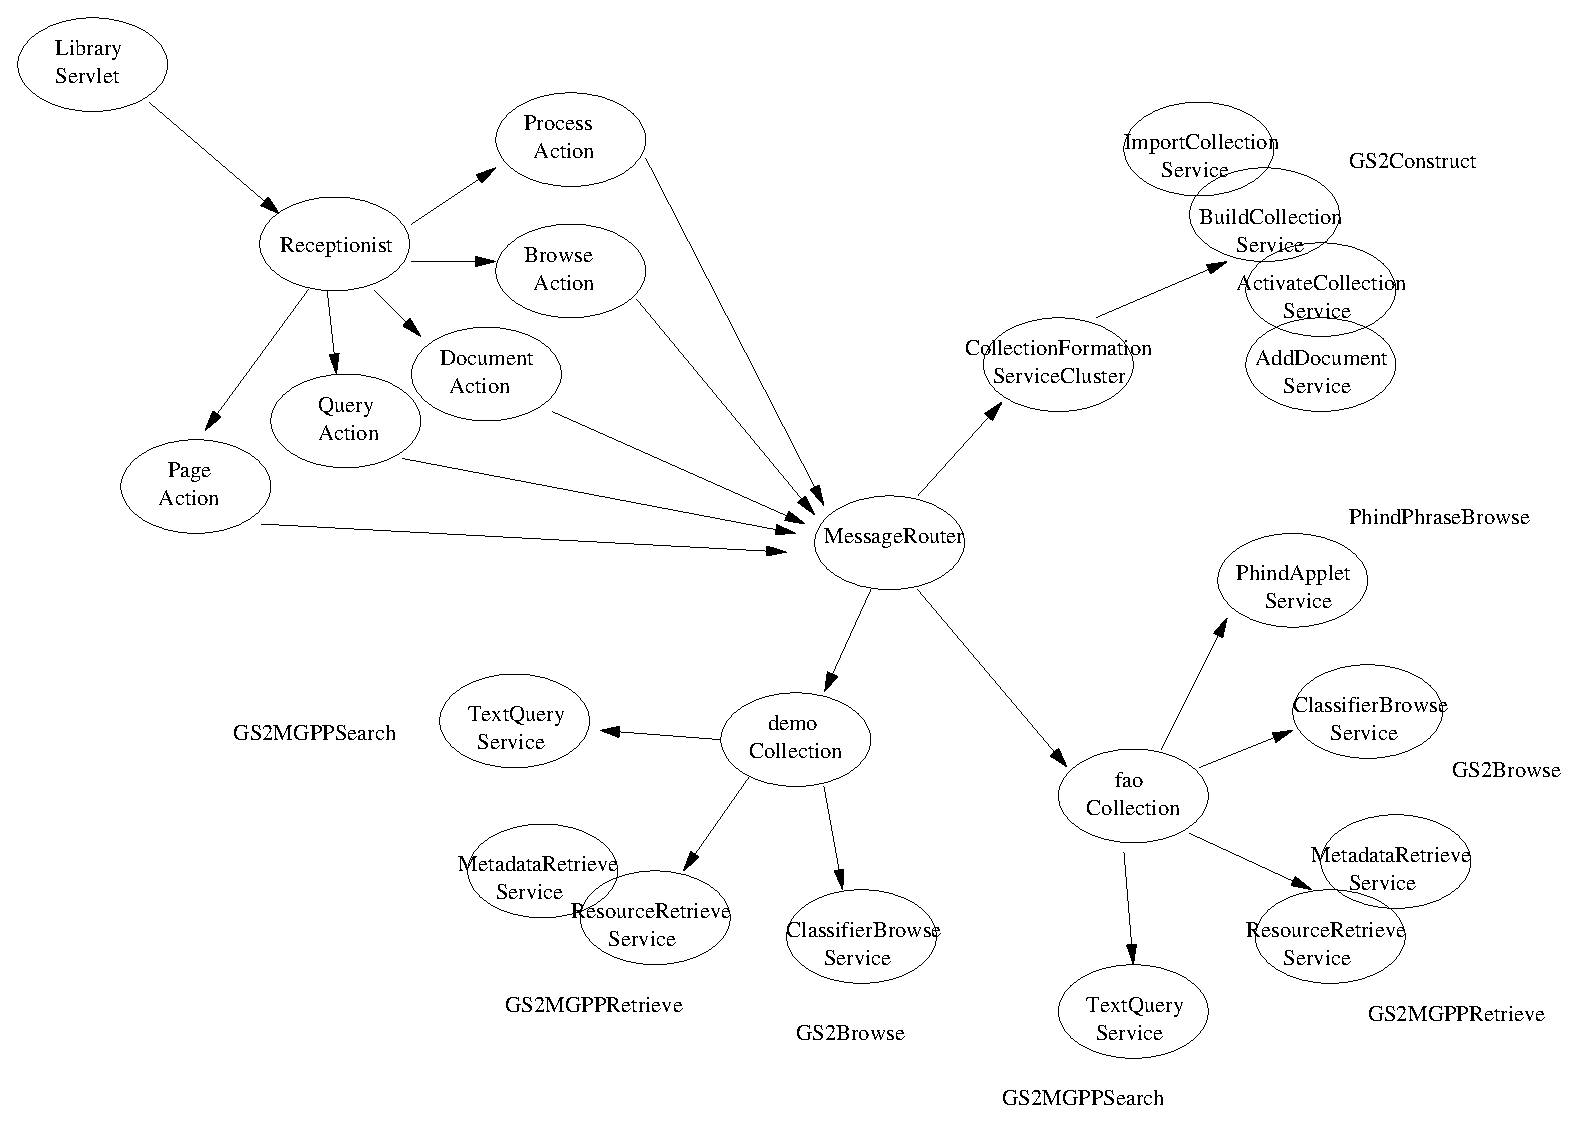
\includegraphics[width=4in]{local} %5.8
  \caption{A simple stand-alone site.}
  \label{fig:local}
\end{figure}


{\em MessageRouter}: this is the central module for a site. It controls the site, loading up all the collections, clusters, communicators needed. All messages pass through the MessageRouter. Communication between remote sites is always done between MessageRouters, one for each site.

{\em Collection and ServiceCluster}: these are very similar, and group a set of services into a conceptual group.. They both provide some metadata about the collection/cluster, and a list of services. The services are provided by ServiceRack objects that the collection/cluster loads up. A Collection is a specific type of ServiceCluster. A ServiceCluster groups services that are related conceptually, e.g. all the building services may be part of a cluster. What is part of a cluster is specified by the site configuration file. A Collection's services are grouped by the fact that they all operate on some common data---the documents in the collection.
Functionally Collection and ServiceCluster are very similar, but conceptually, and to the user, they are quite different.

{\em Service}: these provide the core functionality of the system e.g. searching, retrieving documents, building collections etc. One or more may be grouped into a single Java class (ServiceRack) for code reuse, or to avoid instantiating the same objects several times. For example, MGPP searching services all need to have the index loaded into memory. 

{\em Communicator/Server}: these facilitate communication between remote modules. For example, if you want MR1 to talk to MR2, you need a Communicator-Server pair. The Server sits on top of MR2, and MR1 talks to the Communicator. Each communication type needs a new pair. So far we have only been using SOAP, so we have a SOAPCommunicator and a SOAPServer.

{\em Receptionist}: this is the point of contact for the 'front end'. Its core functionality involves routing requests to the Actions, but it may do more than that. For example, a Receptionist may: modify the request in some way before sending it to the appropriate Action; add some data to the page responses that is common to all pages; transform the response into another form using XSLT. There is a hierarchy of different Receptionist types, which is described in Section~\ref{sec:recepts}.

{\em Actions}: these do the job of creating the 'pages'. There is a different action for each type of page, for example PageAction handles semi-static pages, QueryAction handles queries, DocumentAction displays documents. They know a little bit about specific service types. Based on the 'CGI' arguments passed in to them, they construct requests for the system, and put together the responses into data for the page. This data is returned to the Receptionist, which may transform it to HTML. The various actions are described in  more detail in Section~\ref{sec:pagegen}.


\subsection{Start up configuration}\label{sec:startup-config}

We use the Tomcat web server, which operates either stand-alone in a test mode
or in conjunction with the Apache web server.  The \gs\  LibraryServlet
class is loaded by Tomcat  and the servlet's \gst{init()} method is called.  Each time a
\gst{get/put/post} (etc.) is used, a new thread is started and
\gst{doGet()/doPut()/doPost()} (etc.) is called.

The \gst{init()} method creates a new Receptionist and a new 
MessageRouter. Default classes (DefaultReceptionist, MessageRouter) are used unless subclasses have been specified  in the servlet initiation parameters (see Section~\ref{sec:sites-and-ints}). The appropriate system variables are set for each object (interface
name, site name, etc.) and then \gst{configure()} is called on both. The MessageRouter handle 
is passed to the Receptionist. The servlet then communicates only with
the Receptionist, not with the MessageRouter.

The Receptionist reads in the \gst{interfaceConfig.xml} file (see Section~\ref{sec:interfaceconfig}), and loads up all the different Action classes. Other Actions may be loaded on the fly as needed. Actions are added to a map, with shortnames for keys. Eg the QueryAction is added with key 'q'. The Actions are passed the MessageRouter reference too.
If the Receptionist is a TransformingReceptionist, a mapping between shortnames  and XSLT file names is also created. 

The MessageRouter reads in its site configuration file \gst{siteConfig.xml} (see Section~\ref{sec:siteconfig}). It creates a module map that maps names to objects. This is used for routing the messages. It also keeps small chunks of XML---serviceList, collectionList, clusterList and siteList. These are part of what get returned in response to a describe request (see Section~\ref{sec:describe}.).

Each ServiceRack specified in the configuration file is created, then queried for its list of services. Each service name is added to the map, pointing to the ServiceRack object. Each service is also added to the serviceList. After this stage, ServiceRacks are transparent to the system, and each service is treated as a separate module.

ServiceClusters are created and passed the \gst{<serviceCluster>} element for configuration. They are added to the map as is, with the cluster name as a key. A serviceCluster is also added to the serviceClusterList.

For each site specified, the MessageRouter creates an appropriate type of Communicator object. Then it tries to get the site description. If the server for the remote site is up and running, this should  be successful. The site will be added to the mapping with its site name as a key. The site's collections, services and clusters will also be added into the static xml lists. If the server for the remote site is not running, the site will not be included in the siteList or module map. To try again to access the site, either Tomcat must be restarted, or a run-time reconfigure-site command must be sent (see Section~\ref{sec:runtime-config}).

The MessageRouter also looks inside the site's \gst{collect} directory, and  loads up a Collection object for each valid collection found. If a \gst{collectionInit.xml} file is present, a subclass of Collection may be used.
The Collection object reads its \gst{buildConfig.xml} and \gst{collectionConfig.xml}
files, determines the metadata, and loads ServiceRack classes based on the 
names specified in \gst{buildConfig.xml\/}. The \gst{<serviceRack>} XML element is passed to the object to be used in configuration. The \gst{collectionConfig.xml} contents are also passed in to the ServiceRacks. Any format or display information that the services need must be extracted from the collection configuration file.
Collection objects are added to the module map with their name as a key, and also a collection element is added into the collectionList XML.

\subsection{Message passing}

There are two types of messages used by the system: external and internal messages. All messages have an enclosing \gst{<message>} element, which contains either one or more requests, or one or more responses. In the following descriptions, the message element is not shown, but is assumed to be present.  
Action in \gsiii\  is originated by a request coming in from the outside. In the standard web-based \gs, this comes from a servlet and is passed into the Receptionist. This ``external'' type request is a request for a page of data, and contains a representation of the CGI style arguments. A page of XML is returned, which can be in HTML format or other depending on the output parameter of the request. 

Messages inside the system (``internal'' messages) all follow the same basic format: message elements contain multiple request elements, or multiple response elements. Messaging is all synchronous. The same number of responses as requests will be returned. Currently all requests are independent, so any requests can be combined into the same message, and they will be answered separately, with their responses being sent back in a single message.

When a page request (external request) comes in to the Receptionist, it looks at the action attribute and passes the request to the appropriate Action module. The Action will fire one or more internal requests to the MessageRouter, based on the arguments. The data is gathered into a  response, which is returned to the Receptionist.  The page that the receptionist returns contains the original request, the response from the action and other info as needed (depends on the type of Receptionist). The data may be transformed in some way --- for the \gs\ servlet  we transform using XSLT to generate HTML pages.

Actions send internal style messages to the MessageRouter. Some can be answered by it, others are passed on to collections, and maybe on to services. Internal requests are for simple actions, such as search, retrieve metadata, retrieve document text
There are different internal request types: describe, process, system, format, status. Process requests do the actual work of the system, while the other types get auxiliary information. The format of the requests and responses for each internal request type are described in the following sections. External style requests, and their page responses are described in the Section about page generation (Section~\ref{sec:pagegen}).

\subsection{'describe'-type messages}\label{sec:describe}

The most basic of the internal standard requests is ``describe-yourself'', which can be sent to any module in the system. The module responds with a semi-predefined piece of XML, making these requests very efficient. The response is predefined apart from any language-specific text strings, which are put together as each request comes in, based on the language attribute of the request.
\begin{quote}\begin{gsc}\begin{verbatim}
<request lang='en' type='describe' to=''/>
\end{verbatim}\end{gsc}\end{quote}
If the \gst{to} field is empty, a request is answered by the MessageRouter. 
An example response from a MessageRouter might look like this:
\begin{quote}\begin{gsc}\begin{verbatim}
<response lang='en' type='describe'>
  <serviceList/>
  <siteList>
    <site name='org.greenstone.gsdl1'
            address='http://localhost:8080/greenstone3/services/localsite'
            type='soap' />
  </siteList>
  <serviceClusterList>
    <serviceCluster name="build" />
  </serviceClusterList>
  <collectionList>
    <collection name='org.greenstone.gsdl1/
  	              org.greenstone.gsdl2/fao' />
    <collection name='org.greenstone.gsdl1/demo' />
    <collection name='org.greenstone.gsdl1/fao' />
    <collection name='myfiles' />
  </collectionList>
</response>
\end{verbatim}\end{gsc}\end{quote}
This MessageRouter has no individual site-wide services (an empty \gst{<serviceList>}), but has a service cluster called build (which provides collection importing and building functionality).  It
communicates with one site, \gst{org.greenstone.gsdl1}.  It is aware of four
collections.  One of these, \gst{myfiles}, belongs to it; the other three are
available through the external site.  One of those collections is actually from
a further external site.

It is possible to ask just for a specific part of the information provided by a
describe request, rather than the whole thing. For example, these two
messages get the \gst{collectionList} and the \gst{siteList} respectively: 
\begin{quote}\begin{gsc}\begin{verbatim}
<request lang='en' type='describe' to=''>
  <paramList>
    <param name='subset' value='collectionList'/>
  </paramList>
</request>

<request lang='en' type='describe' to=''>
  <paramList>
    <param name='subset' value='siteList'/>
  </paramList>
</request>
\end{verbatim}\end{gsc}\end{quote}

Subset options for the MessageRouter include \gst{collectionList}, \gst{serviceClusterList}, \gst{serviceList}, \gst{siteList}.

When a collection or service cluster is asked to describe itself, what is returned is a list of metadata, some display elements, and  a list of services.  For example, here is such a message, along with a sample response.

\begin{quote}\begin{gsc}\begin{verbatim}
<request lang='en' type='describe' to='mgppdemo'/>

<response from="mgppdemo" type="describe">
  <collection name="mgppdemo">
    <displayItem lang="en" name="name">greenstone mgpp demo
    </displayItem>
    <displayItem lang="en" name="description">This is a 
      demonstration collection for the Greenstone digital 
      library software. It contains a small subset (11 books) 
      of the Humanity Development Library. It is built with 
      mgpp.</displayItem>
    <displayItem lang="en" name="icon">mgppdemo.gif</displayItem>
    <serviceList>
      <service name="DocumentStructureRetrieve" type="retrieve" />
      <service name="DocumentMetadataRetrieve" type="retrieve" />
      <service name="DocumentContentRetrieve" type="retrieve" />
      <service name="ClassifierBrowse" type="browse" />
      <service name="ClassifierBrowseMetadataRetrieve" 
            type="retrieve" />
      <service name="TextQuery" type="query" />
      <service name="FieldQuery" type="query" />
      <service name="AdvancedFieldQuery" type="query" />
      <service name="PhindApplet" type="applet" />
    </serviceList>
    <metadataList>
      <metadata name="creator">greenstone@cs.waikato.ac.nz</metadata>
      <metadata name="numDocs">11</metadata>  
      <metadata name="buildType">mgpp</metadata>
      <metadata name="httpPath">http://kanuka:8090/greenstone3/sites/
                                localsite/collect/mgppdemo</metadata>
    </metadataList>
  </collection>
</response>
\end{verbatim}\end{gsc}\end{quote}

Subset options for a collection or serviceCluster include \gst{metadataList}, \gst{serviceList}, and \gst{displayItemList}.

This collection provides many typical services. Notice how this response lists the services available, while the collection configuration file for this collection (Figure~\ref{fig:collconfig}) described serviceRacks. Once the service racks have been configured, they become transparent in the system, and only services are referred to.
There are three document retrieval services, for structural information, metadata, and content. The Classifier services retrieve classification structure and metadata. These five services were all provided by the GS2MGPPRetrieve ServiceRack. The three query services were provided by GS2MGPPSearch serviceRack, and provide different kinds of query interface. The last service, PhindApplet, is provided by the PhindPhraseBrowse serviceRack and is an applet service.

A \gst{describe} request sent to a service returns a list of parameters that
the service accepts and some display information, (and in future may describe the content type for the request and response). Subset options for the request include \gst{paramList} and \gst{displayItemList}.

Parameters can be in the following formats:
\begin{quote}\begin{gsc}\begin{verbatim}
<param name='xxx' type='integer|boolean|string|invisible' default='yyy'/>
<param name='xxx' type='enum_single|enum_multi' default='aa'/>
  <option name='aa'/><option name='bb'/>...
</param>
<param name='xxx' type='multi' occurs='4'>
 <param .../>
 <param .../>
</param>
\end{verbatim}\end{gsc}\end{quote}

If no default is specified, the parameter is assumed to be mandatory.
Here are some examples of parameters:
\begin{quote}\begin{gsc}\begin{verbatim}
<param name='case' type='boolean' default='0'/>

<param name='maxDocs' type='integer' default='50'/>

<param name='index' type='enum' default='dtx'>
  <option name='dtx'/>
  <option name='stt'/>
  <option name='stx'/>
<param>

<!-- this one is for the text box and field list for the 
simple field query-->
<param name='simpleField' type='multi' occurs='4'>
  <param name='fqv' type='string'/>
  <param name='fqf' type='enum_single'>
    <option name='TI'/><option name='AU'/><option name='OR'/>
  </param>
</param>

\end{verbatim}\end{gsc}\end{quote}
The type attribute is used to determine how to display the parameters on a web page or interface. For example, a string parameter may result in a text entry box, a boolean an on/off button, enum\_single/enum\_multi a drop-down menu, where one or many items, respectively, can be selected.
A multi-type parameter indicates that two or more parameters are associated, and should be displayed appropriately. For example, in a field query, the text box and field list should be associated. The occurs attribute specifies how many times the parameter should be displayed on the page.
Parameters also come with display information: all the text strings needed to present them to the user. These include the name of the parameter and the display values for any options. These are included in the above parameter descriptions in the form of \gst{<displayItem>} elements.

A service description also contains some display information---this includes the name of the service, and the text  for the submit button. 

Here is a sample describe request to the FieldQuery service of collection mgppdemo, along with its response. The parameters in this example include their display information. Figure~\ref{fig:query-display} shows an example HTML search form that may be generated from this describe response. 

\begin{quote}\begin{gsc}\begin{verbatim}
<request lang="en" to="mgppdemo/FieldQuery" type="describe" />

<response from="mgppdemo/FieldQuery" type="describe">
  <service name="FieldQuery" type="query">
    <displayItem name="name">Form Query</displayItem>
    <displayItem name="submit">Search</displayItem>
    <paramList>
      <param default="Doc" name="level" type="enum_single">
        <displayItem name="name">Granularity to search at</displayItem>
        <option name="Doc">
          <displayItem name="name">Document</displayItem>
        </option>
        <option name="Sec">
          <displayItem name="name">Section</displayItem>
        </option>
        <option name="Para">
          <displayItem name="name">Paragraph</displayItem>
        </option>
      </param>
      <param default="1" name="case" type="boolean">
        <displayItem name="name">Turn casefolding </displayItem>
        <option name="0">
          <displayItem name="name">off</displayItem>
        </option>
        <option name="1">
          <displayItem name="name">on</displayItem>
        </option>
      </param>
      <param default="1" name="stem" type="boolean">
        <displayItem name="name">Turn stemming </displayItem>
        <option name="0">
          <displayItem name="name">off</displayItem>
        </option>
        <option name="1">
          <displayItem name="name">on</displayItem>
        </option>
      </param>
      <param default="10" name="maxDocs" type="integer">
        <displayItem name="name">Maximum documents to return
        </displayItem>
      </param>
      <param name="simpleField" occurs="4" type="multi">
        <displayItem name="name"></displayItem>
        <param name="fqv" type="string">
          <displayItem name="name">Word or phrase </displayItem>
        </param>
        <param default="ZZ" name="fqf" type="enum_single">
          <displayItem name="name">in field</displayItem>
          <option name="ZZ">
            <displayItem name="name">allfields</displayItem>
          </option>	  
          <option name="TX">
            <displayItem name="name">text</displayItem>
          </option>
          <option name="TI">
            <displayItem name="name">Title</displayItem>
          </option>
          <option name="SU">
            <displayItem name="name">Subject</displayItem>
          </option>
          <option name="ORG">
            <displayItem name="name">Organization</displayItem>
          </option>
          <option name="SO">
            <displayItem name="name">Source</displayItem>
          </option>
        </param>
      </param>
    </paramList>
  </service>
</response>
\end{verbatim}\end{gsc}\end{quote}

\begin{figure}[t]
  \centering
  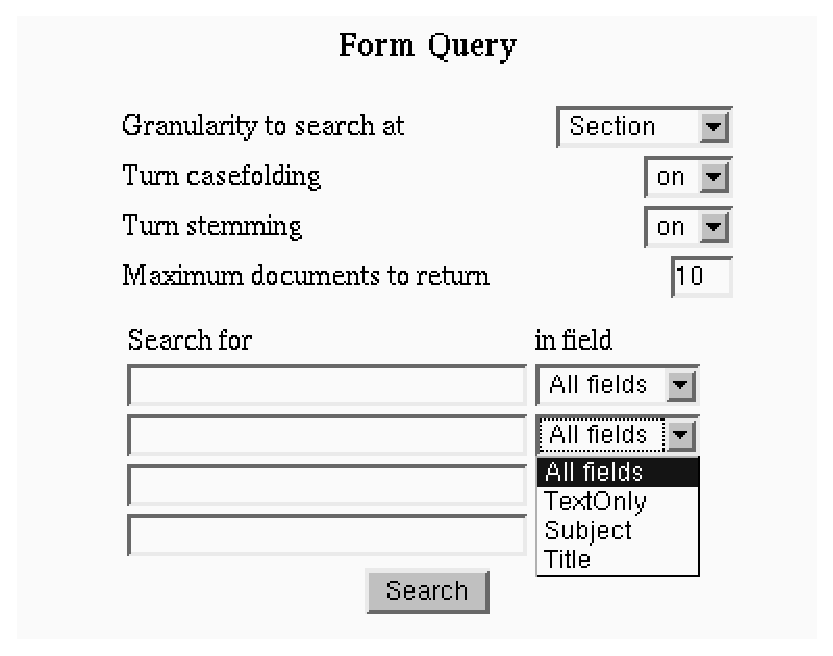
\includegraphics[width=3.5in]{query2}
  \caption{The previous query service describe response as displayed on the search page.}
  \label{fig:query-display}
\end{figure}

A describe request to an applet type service returns the applet HTML element: this will be embedded into a web page to run the applet. 
\begin{quote}\begin{gsc}\begin{verbatim}
<request type='describe' to='mgppdemo/PhindApplet'/>

<response type='describe'>
  <service name='PhindApplet' type='query'>
    <applet ARCHIVE='phind.jar, xercesImpl.jar, gsdl3.jar, 
			jaxp.jar, xml-apis.jar'
            CODE='org.greenstone.applet.phind.Phind.class'
            CODEBASE='lib/java'
            HEIGHT='400' WIDTH='500'>
      <PARAM NAME='library' VALUE=''/>
      <PARAM NAME='phindcgi' VALUE='?a=a&amp;sa=r&amp;sn=Phind'/>
      <PARAM NAME='collection' VALUE='mgppdemo' />
      <PARAM NAME='classifier' VALUE='1' />
      <PARAM NAME='orientation' VALUE='vertical' />
      <PARAM NAME='depth' VALUE='2' />
      <PARAM NAME='resultorder' VALUE='L,l,E,e,D,d' />
      <PARAM NAME='backdrop' VALUE='interfaces/default/>
				      images/phindbg1.jpg'/>
      <PARAM NAME='fontsize' VALUE='10' />
      <PARAM NAME='blocksize' VALUE='10' />
      The Phind java applet.
    </applet>
    <displayItem name="name">Browse phrase hierarchies</displayItem>
  </service>
</response>
\end{verbatim}\end{gsc}\end{quote}

Note that the library parameter has been left blank. This is because library refers to the current servlet that is running and the name is not necessarily known in advance. So either the applet action or the Receptionist must fill in this parameter before displaying the HTML.

\subsection{'system'-type messages}\label{sec:system}

``System'' requests are used to tell a MessageRouter, Collection or ServiceCluster to update its cached information and activate or deactivate other modules. For example, the MessageRouter has a set of Collection modules that it can talk to. It also holds some XML information about those collections---this is returned when a request for a collection list comes in. If a collection is deleted or modified, or a new one created, this information may need to change, and the list of available modules may also change. Currently these requests are initiated by particular CGI requests (see Section~\ref{sec:runtime-config}).

The basic format of a system request is as follows:

\begin{quote}\begin{gsc}\begin{verbatim}
<request type='system' to=''>
  <system .../>
</request>
\end{verbatim}\end{gsc}\end{quote}

One or more actual requests are specified in  system elements. The following are examples:
\begin{quote}\begin{gsc}\begin{verbatim}
<system type='configure' subset=''/>
<system type='configure' subset='collectionList'/>
<system type='activate' moduleType='collection' moduleName='demo'/>
<system type='deactivate' moduleType='site' moduleName='site1'/>
\end{verbatim}\end{gsc}\end{quote}

The first request reconfigures the whole site---the MessageRouter goes through its whole configure process again. The second request just reconfigures the collectionList---the MessageRouter will delete all its collection information, and re-look through the collect directory and reload all the collections again.
The third request is to activate collection demo. This could be a new collection, or a reactivation of an old one. If a collection module already exists, it will be deleted, and a new one loaded. The final request deactivates the site site1---this removes the site from the siteList and module map, and also removes any of that sites collections/services from the static lists.

A response just contains a status message\footnote{TODO: add in error/status codes}, for example:
\begin{quote}\begin{gsc}\begin{verbatim}
<status>MessageRouter reconfigured successfully</status>
<status>Error on reconfiguring collectionList</status>
<status>collection:demo activated</status>
<status>site:site1 deactivated</status>
\end{verbatim}\end{gsc}\end{quote}

System requests are mainly answered by the MessageRouter. However, Collections and ServiceClusters will respond to a subset of these requests. 

\subsection{'format'-type messages}\label{sec:format}

Collection designers are able to specify how their collection looks to a certain degree. They can specify format statements for display that will apply to the results of a search, the display of a document, entries in a classification hierarchy, for example. This info is generally service specific. All services respond to a format request, where they return any service specific formatting information. A typical request and response looks like this:
\begin{quote}\begin{gsc}\begin{verbatim}
<request lang="en" to="mgppdemo/FieldQuery" type="format" />

<response from="mgppdemo/FieldQuery" type="format">
  <format>
    <gsf:template match="documentNode"><td><gsf:link>
      <gsf:metadata name="Title" />(<gsf:metadata name="Source" />)
      </gsf:link></td>
    </gsf:template>
  </format>
</response>
\end{verbatim}\end{gsc}\end{quote}

The actual format statements are described in Section~\ref{sec:formatstmt}. They are templates written directly in XSLT, or in GSF (GreenStone Format) which is a simple XML representation of the more complicated XSLT templates. 
GSF-style format statements need to be converted to proper XSLT. This is currently done by the Receptionist (but may be moved to an ActionHelper): the format XML is transformed to XSLT using XSLT with the config\_format.xsl stylesheet.

\subsection{'status'-type messages}\label{sec:status}

These are only used with process-type services, which are those where a request is sent to start some type of process (see Section~\ref{sec:process}). An initial 'process' request to a 'process' service generates a response which states whether the process had successfully started, and whether its still continuing. If the process is not finished, status requests can be sent repeatedly to the service to poll the status, using the pid to identify the  process.  Status codes are used to identify the state of a process. The values used at the moment are listed in Table~\ref{tab:status codes}\footnote{A more standard set of codes should probably be used, for example, the HTTP codes}.

\begin{table}
\caption{Status codes currently used in \gsiii\ }
\label{tab:status codes}
{\footnotesize
\begin{tabular}{llp{8cm}}
\hline
\bf code name & \bf code  & \bf meaning \\
& \bf value & \\
\hline
SUCCESS &  1 & the request was accepted, and the process was  completed \\
ACCEPTED & 2 & the request was accepted, and the process has been started, but it is not completed yet \\
ERROR & 3 & there was an error and the process was stopped \\
CONTINUING & 10 & the process is still continuing \\
COMPLETED & 11 & the process has  finished \\
HALTED & 12 & the process has stopped  \\
INFO & 20 & just an info message that doesn't imply anything \\
\hline
\end{tabular}}
\end{table}

 The following shows an example status request, along with two responses, the first a 'OK but continuing' response, and the second a 'successfully completed' response. The content of the status elements in the two responses is the output from the process since the last status update was sent back.

\begin{quote}\begin{gsc}\begin{verbatim}
<request lang="en" to="build/ImportCollection" type="status">
  <paramList>
    <param name="pid" value="2" />
  </paramList>
</request>

<response from="build/ImportCollection">
  <status code="2" pid="2">Collection construction: import collection.
command = import.pl -collectdir /research/kjdon/home/greenstone3/web/sites/
    localsite/collect test1
starting
  </status>
</response>

<response from="build/ImportCollection">
  <status code="11" pid="2">RecPlug: getting directory 
/research/kjdon/home/greenstone3/web/sites/localsite/collect/test1/import
WARNING - no plugin could process /.keepme
 
*********************************************
Import Complete
*********************************************
* 1 document was considered for processing
* 0 were processed and included in the collection
* 1 was rejected. See /research/kjdon/home/greenstone3/web/sites/
    localsite/collect/test1/etc/fail.log for a list of rejected documents
Success
  </status>
</response>
\end{verbatim}\end{gsc}\end{quote}

\subsection{'process'-type messages}

Process requests and responses  provide  the major functionality of the system---these are the ones that do the actual work. The format depends on the service they are for, so I'll describe these by service.

Query type services TextQuery, FieldQuery, AdvancedFieldQuery (GS2MGSearch, GS2MGPPSearch), TextQuery (LuceneSearch)
The main type of requests in the system are for services. There are different types of services, currently: \gst{query}, \gst{browse}, \gst{retrieve}, \gst{process}, \gst{applet}, \gst{enrich}. Query services do some kind of search and return a list of document identifiers. Retrieve services can return the content of those documents, metadata about the documents, or other resources. Browse is for browsing lists or hierarchies of documents. Process type services are those where the request is for a command to be run. A status code will be returned immediately, and then if the command has not finished, an update of the status can be requested. Applet services are those that run an applet. Enrich services take a document and return the document with some extra markup added.

  Other possibilities include transform, extract, accrete. These types of service generally enhance the functionality of the first set. They may be used during collection formation: 'accrete' documents by adding them to a collection, 'transform' the documents into a different format, 'extract' information or acronyms from the documents, 'enrich' those documents with the information extracted or by adding new information. They may also be used during querying: 'transform' a query before using it to query a collection, or 'transform' the documents you get back into an appropriate form.

The basic structure of a service 'process' request is as follows:
\begin{quote}\begin{gsc}\begin{verbatim}

<request lang='en'  type='process' to='demo/TextQuery'>
  <paramList/>
  other elements...
</request>

\end{verbatim}\end{gsc}\end{quote}

The parameters are name-value pairs corresponding to parameters that were specified in the service description sent in response to a describe request. 

\begin{quote}\begin{gsc}\begin{verbatim}
<param name='case' value='1'/>
<param name='maxDocs' value='34'/>
<param name='index' value='dtx'/>
\end{verbatim}\end{gsc}\end{quote}

Some requests have other content---for document retrieval, this would be a list of document identifiers to retrieve. For metadata retrieval, the content is the list of documents to retrieve metadata for. 

Responses vary depending on the type of request. The following sections look at the process type requests and responses for each type of service.

\subsubsection{'query'-type services}
Responses to query requests contain a list of document identifiers, along with some other information, dependent on the query type. For a text query, this includes term frequency information, and some metadata about the result. For instance, a text query on 'snail farming', with the parameter 'maxDocs=10' might return the first 10 documents, and one of the query metadata items would be the total number of documents that matched the query.\footnote{no metadata about the query result is returned yet.}

The following shows an example query request and its response.

Find at most 10 Sections in the mgppdemo collection, containing the word snail (stemmed), returning the results in ranked order:
\begin{quote}\begin{gsc}\begin{verbatim}
<request lang='en'  to="mgppdemo/TextQuery" type="process">
  <paramList>
    <param name="maxDocs" value="10"/>
    <param name="queryLevel" value="Section"/>
    <param name="stem" value="1"/>
    <param name="matchMode" value="some"/>
    <param name="sortBy" value="1"/>
    <param name="index" value="t0"/>
    <param name="case" value="0"/>
    <param name="query" value="snail"/>
  </paramList>
</request>

<response from="mgppdemo/TextQuery" type="process">
  <metadataList>
    <metadata name="numDocsMatched" value="59" />
  </metadataList>
  <documentNodeList>
    <documentNode nodeID="HASHac0a04dd14571c60d7fbfd.4.2" 
	docType='hierarchy' nodeType="leaf" />
    <documentNode nodeID="HASH010f073f22033181e206d3b7.2.12" 
	docType='hierarchy' nodeType="leaf" />
    <documentNode nodeID="HASH010f073f22033181e206d3b7.1" 
	docType='hierarchy' nodeType="interior" />
    <documentNode nodeID="HASHac0a04dd14571c60d7fbfd.2.2" 
	docType='hierarchy' nodeType="leaf" />
    ...
  </documentNodeList>
  <termList>
    <term field="" freq="454" name="snail" numDocsMatch="58" stem="3">
      <equivTermList>
        <term freq="" name="Snail" numDocsMatch="" />
        <term freq="" name="snail" numDocsMatch="" />
        <term freq="" name="Snails" numDocsMatch="" />
        <term freq="" name="snails" numDocsMatch="" />
      </equivTermList>
    </term>
  </termList>
</response>
\end{verbatim}\end{gsc}\end{quote}

The list of document identifiers includes some information about document type and node type. Currently, document types include \gst{simple}, \gst{paged} and \gst{hierarchy}. \gst{simple} is for single section documents, i.e. ones with no sub-structure. \gst{paged} is documents that have a single list of sections, while \gst{hierarchy} type documents have a hierarchy of nested sections. For \gst{paged} and \gst{hierarchy} type documents, the node type identifies whether a section is the root of the document, an internal section, or a leaf.

The term list identifies, for each term in the query, what its frequency in the collection is, how many documents contained that term, and a list of its equivalent terms (if stemming or casefolding was used).

\subsubsection{'browse'-type services}

Browse type services are used for classification browsing. The request consists of a list of classifier identifiers, and some structure parameters listing what structure to retrieve.

\begin{quote}\begin{gsc}\begin{verbatim}
<request lang="en" to="mgppdemo/ClassifierBrowse" type="process">
  <paramList>
    <param name="structure" value="ancestors" />
    <param name="structure" value="children" />
  </paramList>
  <classifierNodeList>
    <classifierNode nodeID="CL1.2" />
  </classifierNodeList>
</request>

<response from="mgppdemo/ClassifierBrowse" type="process">
  <classifierNodeList>
    <classifierNode nodeID="CL1">
      <nodeStructure>
	<classifierNode nodeID="CL1">
          <classifierNode nodeID="CL1.2">
	    <classifierNode nodeID="CL1.2.1" />
	    <classifierNode nodeID="CL1.2.2" />
	    <classifierNode nodeID="CL1.2.3" />
	    <classifierNode nodeID="CL1.2.4" />
	    <classifierNode nodeID="CL1.2.5" />
          </classifierNode>	
	</classifierNode>
      </nodeStructure>
    </classifierNode>
  </classifierNodeList>
</response>
\end{verbatim}\end{gsc}\end{quote}

Possible values for structure parameters are \gst{ancestors}, \gst{parent}, \gst{siblings}, \gst{children}, \gst{descendants}. The response gives, for each identifier in the request, a \gst{<nodeStructure>} element with all the requested structure put together into a hierarchy. The structure may include classifier and document nodes. 

Structural info can also be requested in the \gst{paramList}, and will be returned in a \gst{<nodeStructureInfo>} element. (See the section on DocumentStructureRetrieve messages.)  Possible values for info parameters are \gst{numSiblings}, \gst{siblingPosition}, \gst{numChildren}. 

\subsubsection{'retrieve'-type services}

Retrieval services are special in that requests are not explicitly initiated by a user from a form on a web page, but are called from actions in response to other things. This means that their names are hard-coded into the Actions. DocumentContentRetrieve, DocumentStructureRetrieve and DocumentMetadataRetrieve are the standard names for retrieval services for content, structure, and metadata of documents. Requests to each of these include a list of document identifiers. Because these generally refer to parts of documents, the elements are called \gst{<documentNode>}. For the content, that is all that is required. For the metadata retrieval service, the request also needs parameters specifying what metadata is required. For structure retrieval services, requests need parameters specifying what structure or structural info is required.

Some example requests and responses follow.

Give me the Title metadata for these documents:
\begin{quote}\begin{gsc}\begin{verbatim}

<request lang="en" to="mgppdemo/DocumentMetadataRetrieve" type="process">
  <paramList>
    <param name="metadata" value="Title" />
  </paramList>
  <documentNodeList>
    <documentNode nodeID="HASHac0a04dd14571c60d7fbfd.4.2"/>
    <documentNode nodeID="HASH010f073f22033181e206d3b7.2.12"/>
    <documentNode nodeID="HASH010f073f22033181e206d3b7.1"/>
    ...
  </documentNodeList>
</request>

<response from="mgppdemo/DocumentMetadataRetrieve" type="process">
  <documentNodeList>
    <documentNode nodeID="HASHac0a04dd14571c60d7fbfd.4.2">
      <metadataList>
        <metadata name="Title">Putting snails in your second pen</metadata>
      </metadataList>
    </documentNode>
    <documentNode nodeID="HASH010f073f22033181e206d3b7.2.12">
      <metadataList>
        <metadata name="Title">Now you must decide</metadata>
      </metadataList>
    </documentNode>
    <documentNode nodeID="HASH010f073f22033181e206d3b7.1">
      <metadataList>
        <metadata name="Title">Introduction</metadata>
      </metadataList>
    </documentNode>
  </documentNodeList>
</response>
\end{verbatim}\end{gsc}\end{quote}

One or more parameters specifying metadata may be included in a request. Also, a metadata  value of \gst{all} will retrieve all the metadata for each document.

Any browse-type service must also implement a metadata retrieval service to provide metadata for the nodes in the classification hierarchy. The name of it is the browse service name plus \gst{MetadataRetrieve}. For example, the ClassifierBrowse service described in the previous section should also have a ClassifierBrowseMetadataRetrieve service. The request and response format is exactly the same as for the DocumentMetadataRetrieve service, except that \gst{<documentNode>} elements are replaced by \gst{<classifierNode>} elements (and the corresponding list element is also changed).

Give me the text (content) of this document:
\begin{quote}\begin{gsc}\begin{verbatim}
<request lang="en" to="mgppdemo/DocumentContentRetrieve" type="process">
  <paramList />
  <documentNodeList>
    <documentNode nodeID="HASHac0a04dd14571c60d7fbfd.4.2" />
  </documentNodeList>
</request>

<response from="mgppdemo/DocumentContentRetrieve" type="process">
  <documentNodeList>
    <documentNode nodeID="HASHac0a04dd14571c60d7fbfd.4.2">
      <nodeContent>&lt;Section&gt; 
       &lt;/B&gt;&lt;P ALIGN=&quot;JUSTIFY&quot;&gt;&lt;/P&gt;
       &lt;P ALIGN=&quot;JUSTIFY&quot;&gt;190. When the plants in 
       your second pen have grown big enough to provide food and 
       shelter, you can put in the snails.&lt;/P&gt;
      </nodeContent>
    </documentNode>
  </documentNodeList>
</response>
\end{verbatim}\end{gsc}\end{quote}

The content of a node is returned in a \gst{<nodeContent>} element. In this case it is escaped HTML.

Give me the ancestors and children of the specified node, along with the number of siblings it has:
\begin{quote}\begin{gsc}\begin{verbatim}
<request lang="en" to="mgppdemo/DocumentStructureRetrieve" type="process">
  <paramList>
    <param name="structure" value="ancestors" />
    <param name="structure" value="children" />
    <param name="info" value="numSiblings" />
  </paramList>
  <documentNodeList>
    <documentNode nodeID="HASHac0a04dd14571c60d7fbfd.4.2" />
  </documentNodeList>
</request>

<response from="mgppdemo/DocumentStructureRetrieve" type="process">
  <documentNodeList>
    <documentNode nodeID="HASHac0a04dd14571c60d7fbfd.4.2">
      <nodeStructureInfo>
        <info name="numSiblings" value="2" />
      </nodeStructureInfo>
      <nodeStructure>
        <documentNode nodeID="HASHac0a04dd14571c60d7fbfd" 
                docType='hierarchy' nodeType="root">
          <documentNode nodeID="HASHac0a04dd14571c60d7fbfd.4" 
                  docType='hierarchy' nodeType="interior">
            <documentNode nodeID="HASHac0a04dd14571c60d7fbfd.4.2" 
                   docType='hierarchy' nodeType="leaf" />
          </documentNode>
        </documentNode>
      </nodeStructure>
    </documentNode>
  </documentNodeList>
</response>
\end{verbatim}\end{gsc}\end{quote}

Structure is returned inside a \gst{<nodeStructure>} element, while structural info is returned in a \gst{<nodeStructureInfo>} element. Possible values for structure parameters are as for browse services: \gst{ancestors}, \gst{parent}, \gst{siblings}, \gst{children}, \gst{descendants}, \gst{entire}. Possible values for info parameters are \gst{numSiblings}, \gst{siblingPosition}, \gst{numChildren}. 

\subsubsection{'process'-type services}\label{sec:process}
Requests to process-type services are not requests for data---they request some action to be carried out, for example, create a new collection, or import a collection. The response is a status or an error message. The import and build commands may take a long time to complete, so a response is sent back after a successful start to the command. The status may be polled by the requester to see how the process is going. 

Process requests generally contain just a parameter list. Like for any service, the parameters used by a process-type service can be obtained by a describe request to that service.

Here are two example requests for process-services that are part of the build service cluster (hence the addresses all begin with 'build/'), followed by an example response:

\begin{quote}\begin{gsc}\begin{verbatim}
<request lang='en'  type='process' to='build/NewCollection'>
  <paramList>
    <param name='creator' value='me@home.com'/>
    <param name='collName' value='the demo collection'/>
    <param name='collShortName' value='demo'/>
  </paramlist>
</request>

<request lang='en'  type='process' to='build/ImportCollection'>
  <paramList>
    <param name='collection' value='demo'/>
  </paramlist>
</request>

<response from="build/ImportCollection">
  <status code="2" pid="2">Starting process...</status>
</response>
\end{verbatim}\end{gsc}\end{quote}

The \gst{code} attribute in the response specifies whether the command has been successfully stated, whether its still going, etc (see Table~\ref{tab:status codes} for a list of currently used codes). The pid attribute specifies a process id number that can be used when querying the status of this process. The content of the status element is (currently) just the output from the process so far. Status messages, which were described in Section~\ref{sec:status}, are used to find out how the process is going, and whether it has finished or not.

\subsubsection{'applet'-type services}

Applet-type services are those that process the data for an applet. A request consists only of a list of parameters, and the response contains an \gst{<appletData>} element that contains the XML data to be returned to the applet. The format of this is entirely specific to the applet---there is no set format to the applet data.

Here is an example request and response, used by the Phind applet:
\begin{quote}\begin{gsc}\begin{verbatim}
  <request type='query' to='mgppdemo/PhindApplet'>
    <paramList>
      <param name='pc' value='1'/>
      <param name='pptext' value='health'/>
      <param name='pfe' value='0'/>
      <param name='ple' value='10'/>
      <param name='pfd' value='0'/>
      <param name='pld' value='10'/>
      <param name='pfl' value='0'/>
      <param name='pll' value='10'/>
    </paramList>
  </request>

  <response type='query' from='mgppdemo/PhindApplet'>
    <appletData>
      <phindData df='9' ef='46' id='933' lf='15' tf='296'>
        <expansionList end='10' length='46' start='0'>
          <expansion df='4' id='8880' num='0' tf='59'>
            <suffix> CARE</suffix>
          </expansion>
          ...
        </expansionList>
        <documentList end='10' length='9' start='0'>
          <document freq='78' hash='HASH4632a8a51d33c47a75c559' num='0'>
            <title>The Courier - N??159 - Sept- Oct 1996 Dossier Investing 
                   in People Country Reports: Mali ; Western Samoa
            </title>
          </document>
          ...
        </documentList>
        <thesaurusList end='10' length='15' start='0'>
          <thesaurus df='7' id='12387' tf='15' type='RT'>
            <phrase>PUBLIC HEALTH</phrase>
          </thesaurus>...
        </thesaurusList>
      </phindData>
    </appletData>
  </response>

\end{verbatim}\end{gsc}\end{quote}

\subsubsection{'enrich'-type services}

Enrich services typically take some text of documents (inside \gst{<nodeContent>} tags) and returns the text marked up in some way. One example of this is the GatePOSTag service: this identifies Dates, Locations, People and Organizations in the text, and annotates the text with the labels. In the following example, the request is for Location and Dates to be identified.

\begin{quote}\begin{gsc}\begin{verbatim}
<request lang="en" to="GatePOSTag" type="process">
  <paramList>
    <param name="annotationType" value="Date,Location" />
  </paramList>
  <documentNodeList>
    <documentNode nodeID="HASHac0a04dd14571c60d7fbfd">
      <nodeContent>
        FOOD AND AGRICULTURE ORGANIZATION OF THE UNITED NATIONS
        Rome 1986
        P-69
        ISBN 92-5-102397-2
        FAO 1986
      </nodeContent>
    </documentNode>
  </documentNodeList>
</request>

<response from="GatePOSTag" type="process">
  <documentNodeList>
    <documentNode nodeID="HASHac0a04dd14571c60d7fbfd">
      <nodeContent>
	FOOD AND AGRICULTURE ORGANIZATION OF THE UNITED NATIONS
	<annotation type="Location">Rome</annotation> 
        <annotation type="Date">1986</annotation>
        P-69
        ISBN 92-5-102397-2
        FAO <annotation type="Date">1986</annotation>
      </nodeContent>
    </documentNode>
  </documentNodeList>
</response>
\end{verbatim}\end{gsc}\end{quote}

\subsection{Page generation}\label{sec:pagegen} 

A 'page' is some XML or HTML (or other?) data returned in response to an 
external 'page'-type request. These requests originate from outside \gs\ , for example from a servlet, or Java application, and are received by the Receptionist. As described below in Section~\ref{sec:page-requests}, the requests are XML representations of \gs\  URLs. One of the arguments is action (a). This tells the Receptionist which Action module to pass the request to. 

Action modules decode the rest of the arguments to determine what requests need to be made to the system. One or more internal requests may be made to the MessageRouter. A request for format information from the Collection/Service may also be made. The resulting data is gathered together into a single XML response, \gst{<page>}, and returned to the Receptionist. 

The page format is described in Section~\ref{sec:page-format}. The XML may be returned as is, or may be modified by the Receptionist. The various Receptionists are described in Section~\ref{sec:recepts}. The default receptionist used by a servlet transforms the XML into HTML using XSL stylesheets. Section~\ref{sec:collformat} looks at collection specific formatting, in particular for HTML output.
Sections~\ref{sec:pageaction} to \ref{sec:systemaction} look at the various actions and what kind of data they gather.

\subsubsection{'page'-type requests and their arguments}\label{sec:page-requests}

These are requests for a 'page' of data---for example, the home page for a site; the query page for a collection; the text of a document. They contain, in XML, a list of arguments specifying what type of page is required. If the external context is a servlet, the arguments represent the 'CGI' arguments in a \gs\  URL.  The two main arguments are \gst{a} (action) and \gst{sa} (subaction). All other arguments are encoded as parameters.

Here are some examples of  requests\footnote{In a servlet context, these correspond to the arguments \gst{a=p\&sa=about\&c=demo\&l=fr}, and \gst{a=q\&l=en\&s=TextQuery\&c=demo\&rt=r\&ca=0\&st=1\&m=10\&q=snail}.}:

\begin{quote}\begin{gsc}\begin{verbatim}
<request type='page' action='p' subaction='about'
         lang='fr' output='html'>
  <paramList>
    <param name='c' value='demo'/>
  </paramList>
</request>
\end{verbatim}\end{gsc}\end{quote}

\begin{quote}\begin{gsc}\begin{verbatim}
<request type='page' action='q' lang='en' output='html'>
  <paramList>
    <param name='s' value='TextQuery'/>
    <param name='c' value='demo'/>
    <param name='rt' value='r'/>
    <!-- the rest are the service specific params -->
    <param name='ca' value='0'/> <!-- casefold -->
    <param name='st' value='1'/> <!-- stem -->
    <param name='m' value='10'/> <!-- maxdocs -->
    <param name='q' value='snail'/> <!-- query string -->
  </paramList>
</request>
\end{verbatim}\end{gsc}\end{quote}

There are some standard arguments used in Greenstone, and they are described in Table~\ref{tab:args}. These are used by Receptionists and Actions. The GSParams class specifies all the general basic arguments, and whether they should be saved or not (Some arguments need to be saved during a session, and this needs to be implemented outside \gs\  proper --- currently we do this in the servlet, using servlet session handling). The servlet has an init parameter \gst{params\_class} which specifies which params class to use: GSParams can be subclassed if necessary. The Receptionist and Actions must not have conflicting argument names.

Other arguments are used dynamically and come from the Services. Service arguments must always be saved during a session. Services may be created by different people, and may reside on a different site. There is no guarantee that there is no conflict with argument names between services and actions. Therefore service parameters are namespaced when they are put on the page, whereas interface (receptionist and action) parameters have no namespace. The default namespace is s1 (service1) --- any parameters that are for the service will be prefixed by this. For example, the case parameter for a search will be put in the page as s1.case, and the resulting argument in a search URL will be s1.case. When actions are deciding which parameters need to be sent in a request to a service, they can use the namespace information.

If there are  two or more services combined on a page with a single submit button, they will use namespaces s1, s2, s3 etc as needed. The s  (service) parameter will end up with a list of services. For example, \gst{s=TextQuery,MusicQuery,} and the order of these determines the mapping order of the namespaces, i.e. s1 will map to TextQuery, s2 to MusicQuery.

\begin{table}
{\footnotesize
\begin{tabular}{lll}
\hline
\bf Argument & \bf Meaning &\bf Typical values \\
\hline
a & action & a (applet), q (query), b (browse), p (page), pr (process) \\
& & s (system)\\
sa & subaction & home, about (page action)\\
c & collection or  & demo, build \\
& service cluster \\
s & service name & TextQuery, ImportCollection \\
rt & request type & d (display), r (request), s (status) \\
ro & response only & 0 or 1 - if set to one, the request is carried out \\
& & but no processing of the results is done \\
& & currently only used in process actions \\
o & output type & XML, HTML, WML \\
l & language & en, fr, zh ...\\
d & document id & HASHxxx \\
r & resource id & ???\\
pid & process handle & an integer identifying a particular process request \\
\hline
\end{tabular}}
\caption{Generic arguments that can appear in a \gs\  URL}
\label{tab:args}
\end{table}

\subsubsection{page format}\label{sec:page-format}

The basic  page format  is:
\begin{quote}\begin{gsc}\begin{verbatim}
<page lang='en'>
  <pageRequest/>
  <pageResponse/>
</page>
\end{verbatim}\end{gsc}\end{quote}

* show configuration and describe whats its used for

There are two main elements in the page: pageRequest, pageResponse. The pageRequest is the original request that came into the Receptionist---this is included so that any parameters  can be preset to their previous values, for example, the query options on the query form. The pageResponse contains all the data that has been gathered from the system by the action. The other two elements contain extra information needed by XSLT. Config contains run-time variables such as the location of the gsdl home directory, the current site name, the name of the executable that is running (e.g. library)---these are needed to allow the XSLT to generate correct HTML URLs. Display contains some of the text strings needed in the interface---these are separate from the XSLT to allow for internationalization.

The following subsections outline, for each action, what data is needed and what requests are generated to send to the system. 


Once the XML page has been put together, the page to return to the user is created by transforming the XML using XSLT. The output is HTML at this stage, but it will be possible to generate alternative outputs, such as XML, WML etc. A set of XSLT files defines an 'interface'. Different users can change the look of their web pages by creating new XSLT files for a new 'interface'. Just as we have a sites directory where different sites 'live' (ie where their configuration file and collections are located), we have an interfaces directory where the different interfaces 'live' (ie their transforms and images are located there). The default XSLT files are
located in interfaces/default/transforms. Collections, sites and other interfaces
can override these files by having their own copy of the appropriate
files. New interfaces have their own directory inside interfaces/. Sites and collections can have a transform directory containing XSLT files. The order in which the XSLT files are looked for is collection, site, current
interface, default interface.\footnote{this currently breaks down for remote sites - need to rethink it a bit.}
[TODO: describe a bit more?? currently only can get this locally]

\subsubsection{Receptionists}\label{sec:recepts}

The receptionist is the controlling module for the page generation part of \gs\ . It has the job of loading up all the actions, and it knows about the message router it and the actions are supposed to talk to. It routes messages received to the appropriate action (page-type messages) or directly to the message router (all other types). Receptionists also do other things, for example, adding to the page received back from the action any information that is common to all pages.

There are different ways of providing an interface to \gs\ , from web based CGI style (using servlets) to Java GUI applications. These different interfaces require slightly different responses from a receptionist, so we provide several standard types of receptionist.

Receptionist: This is the most basic receptionist. The page it returns consists of the original request, and the response from the action it was sent to. Methods preProcessRequest, and postProcessPage are called on the request and page, respectively, but in this basic receptionist, they don't do anything.

TransformingReceptionist: This extends Receptionist, and overwrites postProcessPage to transform the page using XSLT. An XSLT is listed for each action in the receptionists configuration file, and this is used to transform the page. First, some display information, and configuration information is added to the page. Then it is transformed using the specified XSLT for the action, and returned.

WebReceptionist: The WebReceptionist extends TransformingReceptionist. It doesn't do much else except some argument conversion. To keep the URLs short, parameters from the services are given shortnames, and these are used in the web pages. 

DefaultReceptionist: This extends WebReceptionist, and is the default one for \gsiii\  servlets. Due to the page design, some extra information is needed for each page: some metadata about the current collection. The receptionist sends a describe request to the collection to get this, and appends it to the page before transformation using XSLT.

By default, the LibraryServlet uses DefaultReceptionist. However, there is a servlet init-param called \gst{receptionist} which can be set to make the servlet use a different one.

\subsubsection{Collection specific formatting}\label{sec:collformat}
get format info, transform gsf->xsl. transform xml->html

configuration params are passed in to the transformation
\subsubsection{CGI arguments}


\subsubsection{Page action}\label{sec:pageaction}

PageAction is responsible for displaying kinds of information pages, such as the home page of the library, or the home page of a collection, or the help and preferences pages. These pages are not associated with specific services like the other page types. In general, the data comes from describe requests to various modules.
The different pages are requested using the subaction argument. For the 'home' page, a 'describe' request is sent to the MessageRouter---this returns a list of all the collections, services, serviceClusters and sites known about. For each collection, its metadata is retrieved via a 'describe' request. This metadata is added into the previous result, which is then added into the page.    For the 'about' page, a \gst{describe} request is sent to the module that the about page is about: this may be a collection or a service cluster.  This returns a list of metadata
and a list of services.

To get an external html page embedded into a greenstone collection, i.e. a two frame page, with the top frame containing the collection header and navigation bar, and the second frame containg the external page, use subaction html.
A url would look like
a=p\&amp;sa=html\&amp;c=collname\&amp;url=externalurl

\subsubsection{Query action}\label{sec:queryaction}

The basic URL is \gst{a=q\&s=TextQuery\&c=demo\&rt=d/r}.
There are three query services which have been implemented: TextQuery, FieldQuery, and AdvancedFieldQuery. These are all handled in the same way by query action.
For each page, the service description is requested from the  service  of the current collection (via a describe request).  This is currently done every time the query page is
displayed, but should be cached. The description includes a list of the parameters available for the query, such as case/stem, max num docs to return, etc. If the request type (rt) parameter is set to d for display, the action only needs to display the form, and this is the only request to the service. Otherwise, the submit button has been pressed, and a query request to the TextQuery service is sent. This has  all the parameters from the URL put into the parameter list. A list of document identifiers
is returned. A followup query is sent to the MetadataRetrieve service of the collection: the content includes the list of
documents, with a request for some of their metadata. Which metadata to retrieve is determined by looking through the XSLT that will be used to transform the page. The service description and query result are combined into a page of XML, which is returned to the Receptionist.

\subsubsection{Applet action}\label{sec:appletaction}

There are two types of request to the applet action: \gst{a=a \& rt=d\/} and
\gst{a=a \& rt=r\/}.  The value \gst{rt=d\/} means ``display the applet.'' A
\gst{describe} request is sent to the service, which returns the \gst{<applet>} HTML element.  The transformation file \gst{applet.xsl} embeds this
into the page, and the servlet returns the HTML.

The value \gst{rt=r} signals a request from the applet. A process request containing all the parameters is sent to the applet service. The result contains an appletData element, which contains a single  element - this element is returned
directly to the applet, in XML. No transformation is done. 
Because the AppletAction doesn't know or care anything about the applet data, it can work with any applet-service pair.

Note that the applet HTML may need to know the name of the \gst{library}
program.  However, that name is chosen by the person who installed the software
and will not necessarily be ``library''.  To get around this, the applet can
put a parameter called ``library'' into the applet data with a null value:
\begin{quote}\begin{gsc}\begin{verbatim}
<PARAM NAME='library' VALUE=''/>
\end{verbatim}\end{gsc}\end{quote}
When the AppletAction encounters this parameter it inserts the name of the
current library servlet as its value.

\subsubsection{Document action}\label{sec:documentaction}

DocumentAction is responsible for displaying a document to the user. The display might involve some metadata and/or text for a document or part of a document. For hierarchical documents, a table of contents may be shown, while for paged documents (those with a single linear list of sections), next and previous page buttons may be shown. These different display types require different information about the document. Depending on the arguments, DocumentAction will send requests to several services: DocumentMetadataRetrieve, DocumentStructureRetrieve and DocumentContentRetrieve.

A basic display, for example, Title and text, involves a metadata request to get the Title, and a content request to get the text. Hierarchical table of contents display requires a structure request. If the entire contents is to be displayed, the parameter \gst{structure=entire} would be sent in the request. Otherwise, parameters \gst{structure=ancestors}, \gst{structure=children} and possibly \gst{structure=siblings} may be used, depending in the position of the current node in the document. These return a hierarchical structure of nodes, containing ancestor nodes, child nodes and sibling nodes, respectively.
For paged display, the structure is not actually needed. A structure request is still sent, but this time it requests some information, rather the structure itself. The information requested includes the number of siblings and the current position of the current node, or the number of children (if the current node is the root of the document).

Metadata may be requested for the current node, or for any nodes in the structure, and content also. The metadata and content are added into the appropriate nodes in the structure hierarchy, and this is returned as the page data.

\subsubsection{XML Document action}\label{sec:xmldocumentaction}

XMLDocumentAction is a little different to the standard DocumentAction. It operates in two modes, \gst{text} and \gst{toc}. In \gst{text} mode, it will retrieve the content of the current document node using a DocumentContentRetrieve request. In \gst{toc} mode, it retrieves the entire table of contents for the document using a DocumentStructureRetrieve request. Either mode may also retrieve metadata for the current section or each section in the table of contents.

\subsubsection{GS2Browse action}\label{sec:browseaction}

GS2BrowseAction is for displaying \gsii\  style classifiers. 
\subsubsection{System action}\label{sec:systemaction}

SystemAction allows for manual reconfiguration of various components at run-time. There is no interactive web-page displaying the options, it merely turns a set of CGI arguments into an XML system request. The response from a system request is a message which is displayed to the user.

\begin{table}
\caption{Configure CGI arguments}
\label{tab:system-cgi}
{\footnotesize
\begin{tabular}{ll}
\hline
\bf arg & \bf description\\
\hline
a=s & system action\\
sa=c$|$a$|$d & type of system request: c (configure), a (add/activate), \\
& d (delete/deactivate) \\
c=demo &  the request will go to this collection/servicecluster \\
& instead of the message router\\
ss=collectionList & subset for configure: only reconfigure this part.\\
&  For the MessageRouter,  can be serviceClusterList, serviceList, \\
& collectionList, siteList.\\
&  For a collection/cluster, can be metadataList or serviceList.\\
sn=demo & \\
st=collection& \\
\hline
\end{tabular}}
\end{table}


\subsection{Other code information}

Greenstone has a set of Utility classes, which are briefly described in Table~\ref{tab:utils}.

\begin{table}[h]
\caption{The utility classes in org.greenstone.gsdl3.util}
\label{tab:utils}
{\footnotesize
\begin{tabular}{lp{3.75in}}
\hline
\bf Utility class & \bf Description\\
\hline
CollectionClassLoader & ClassLoader that knows about a collection's resource directory \\
DBInfo & Class to hold info from GDBM database entry \\
Dictionary & wrapper around a Resource Bundle, providing strings with parameters\\
GDBMWrapper & Wrapper for GDBM database. Uses JavaGDBM\\
GSConstants & holds some constants used for servlet arguments and configuration variables\\
GSEntityResolver & an EntityResolver which can be used to find resources such as DTDs\\
GSFile & class to create all \gs\  file paths e.g. used to locate configuration files, XSLT files and collection data. \\
GSHTML & provides convenience methods for dealing with HTML, e.g. making strings HTML safe\\
GSParams & contains names and default values for interface parameters\\
GS2Params & a subclass of GSParams which holds default service parameters too, necessary for the gs2 style interface.\\
GSPath & used to create, examine and modify message address paths\\
GSStatus & some static codes for status messages\\ 
GSXML & lots of methods for extracting information out of \gs\  XML, and creating some common types of elements. Also has static Strings for element and attribute names used by \gs\ .\\
GSXSLT & some manipulation functions for \gs\  XSLT\\
GlobalProperties & Holds the global properties (from global.properties) \\
MacroResolver & Used with replace elements in collection configuration files, replaces a macro or string with another string, metadata or text from a dictionary\\
GS2MacroResolver & MacroResolver for GS2 collections, that uses the GDBM database\\
Misc & miscellaneous functions\\
MyNodeList & A simple implementation of an XML NodeList\\
OID & class to handle \gs\  (2) OIDs\\
Processing & Runs an external process and prints the output from the process \\
SQLQuery & contains a connection to a SQL database, along with some methods for accessing the data, such as converting MG numbers to and from Greenstone OIDs.\\
XMLConverter & provides methods to create new Documents, parse Strings or Files into Documents, and convert Nodes to Strings\\
XMLTransformer & methods to transform XML using XSLT \\
XSLTUtil & contains static methods to be called from within XSLT \\
\hline
\end{tabular}}
\end{table}


\newpage
\section{Developing \gsiii\ : Adding new features}\label{sec:new-features}

[TODO: finish this section ]

\subsection{Creating and using new services}\label{sec:new-services}

There are three parts to adding new services to \gsiii: defining the new service, specifying that it should be loaded, and using it. If you are talking to \gs\ using the SOAP interface, then the firsttwo  parts are all that need to be done. If you are using the Greenstone servlet interface, then you may need to do work for the third part, depending on what kind of new service it is.
If you are adding a service of a type that is already present, for example, a new query service, then the query action can just use your new service as is (assuming it is set up in the same way as the standard query services).
However, if it is a new type of service that the interface and actions don't know about, you willl need to add a new action or modify an existing one so that your service is actually used.

\subsubsection{Creating the service}

You will need to write a new Java class which inherits from \gst{org.greenstone.gsdl3.service.ServiceRack} (or a subclass of this). The class will need to implement at least the \gst{configure}, \gst{process<ServiceName>} and \gst{getServiceDescription} methods. There is a dummy class called \gst{MyNewServicesTemplate.java} in \gst{greenstone3/resources/java} which describes these methods and what needs to be done.

\gst{ServiceRack.java} handles the main \gst{process} method. If the request type is 'describe', then it will send back a copy of short\_service\_info, which contains a list of services. If there request type is describe, but for a particular service, then it will call \gst{getServiceDescroption} for that service. For a format request, it will send any format element found in format\_info\_map for that service. For a processing request to a service, then the \gst{process<ServiceName>} method will be called.

Once the class is written, it needs to be compiled up and either included in one of the existing jar files, or added in as a jar file to \gst{greenstone3/web/WEB-INF/lib} or a class file to \gst{greenstone3/web/WEB-INF/classes}.

\subsubsection{Loading the service}

To have the library load in your new service, it needs to be specified in a configuration file somewhere. For a collection service, add a new \gst{<serviceRack>} element to the collection's \gst{buildConfig.xml} file. This element should contain any information that the class needs to configure its service(s). For a site-wide service, add the \gst{<serviceRack>} element to the site's \gst{siteConfig.xml} file, either in the \gst{serviceRackList} or as part of a \gst{serviceCluster}.

\subsubsection{Using the service}

If you are using the SOAP web service, then you can send an XML request directly to the service. The 'address' of the request will be the service name if it is a site-wide service, cluster-name/service-name if it is site-wide but belonging to a cluster, or collection-name/service-name if it belongs to a collection. You will need to know the format of the XML request and response that the service expects and returns.

If you want to access your new service through the current servlet interface that uses actions, then whether you need to do more work or not depends on whatkind of service you have implemented. If you have written a new query or browse service, for example, that has teh same request and response format as the existing services, then you don't need to do anything else. Your collection can just use the new query service straight away.
If the service is of an existing type, but needs soemthing different in the request/response format, then you may need to modify an existing action to supply or use the new information.
If the service is of a completely new type, then you will probably need a new action to talk to the service and display the results.


\subsection{creating new actions/pages}\label{sec:new-pages}

\subsection{new interfaces}\label{sec:new-interfaces}

It is easy to create new interfaces to \gsiii. Here we are talking about interfaces other than those to display in typical browser.

Handheld devices: Use the standard servlet setup, but with a different set of XSLT files to format the pages for small screens, or use WML.

Java GUI Interface: There are couple of alternatives. Depending on what you want to display in the GUI, you could talk to either a Receptionist or a MessageRouter. The library classes can be set up and compiled into the GUI program.
Talking to a Receptionist will give you access to pages of XML. It is likely that the standard Receptionist class would be used - this doesn't transform the data to HTML. Queries such as ``give me the home page of a collection'' and ``do the following search'' can be issued. All the data needed for the result view is returned. Queries are quite simple, but are limited to what kinds of Actions are available in the library. 
Talking to a MessageRouter requires a bit more effort on the part of the GUI program, but results in greater flexibility. The kinds of queries that can be issued are individual units of action, such as ``describe yourself'', ``search'', ``retrieve the content for this document''. More than one request may need to be made for a particular feature of the GUI. However you can ask for any combination of data available in the system, you are not relying on Actions. What you will implement though, may be a lot like the Action code in terms of request sequences.

Interfaces in other programming languages: Because the communication is all XML based, other interfaces can talk to the Java library if a communication protocol is set up. This could be done using SOAP for example. Like for Java GUI interfaces, the program could talk to a Receptionist or to a MessageRouter. 
e.g. Java interface. where you can interface to. MR vs Receptionist. different receptionists. e.g., handheld - using servlet, transforming recpt, but new set of XSLT Java program other program - talk to recpt but just get back XML data for pages. Java gui - just talk to MR, do all processing itself.

Remote interfaces: remote interfaces can be set up in the same way as above, using a communication protocol between the interface, and the library program.


\subsection{New types of collections}\label{sec:new-coll-types}

The standard type of collection is built with the \gsii\ Perl collection building system. There are many options to this, but it is conceivable that these options don't meet the needs of all collection builders. \gsiii\  has an ability to use any type of collection you can come up with, assuming some Java code is provided. 

There are four levels of customization that may be needed with new collections: service, collection, interface XSLT, and action levels. We will use the example collections that come with \gs\  to describe these different levels.

Firstly, new service classes need to be written to provide the functionality to search/browse/whatever the collection. If the services have similar interfaces and functionality to the standard services, this may be all that is needed. For example, MGPP collections were the first to be served in \gsiii\ . When we came to do MG collections, all we had to do was write some new service classes that interacted with MG instead of MGPP. Because these collections used the same type of services, this was all we had to do. The format of the configuration files was similar, they just specified MG serviceRack classes rather than MGPP ones.

The XML Sample Texts (gberg) collection, however, was done quite differently to the standard collections. New services were provided to search the database (built with Lucene) and to provide the documents and parts of documents (using XSLT to transform the raw XML files). The collectionConfig file had some extra information in it: a list of the documents in the collection along with their Titles. Because the standard collection class has no notion of document lists, a new class was created (org.greenstone.gsdl3.collection.XMLCollection). This class is basically the same as a standard collection class except that it looks for and stores in memory the documentList from the collectionConfig file.

To tell \gs\  to load up a different type of collection class, we use another configuration file: \gst{etc/collectionInit.xml}. This specifies the name of the collection class to use.
Currently, this is all that is specified in that file, but you may want to add parameters for the class etc.

\gst{<collectionInit class="XMLCollection"/>}

The display for the collection is also quite different. The home page for the collection  displays the list of documents. To achieve this, the describe response from the collection had to include the list, and a new XSLT was written for the collection that displayed this. Collection XSLT should be put in the transform directory of the collection\footnote{These are currently only used when running \gs\  in a non-distributed fashion, but it will be added in properly at some stage}.

Document display is  significantly different to standard \gs\ . There are two modes of display: table of contents mode, and content mode. Clicking on a document link from the collection home page takes the user to the table of contents for the collection. Clicking on one of the sections in the table of contents takes them to a display of that section. To facilitate this, not only do we need new XSLT files , we also needed a new action. XMLDocumentAction was created, that used two subactions, toc and text, for the different modes of display.

The Receptionist was told about this new action by the addition of the following element to the interfaceConfig.xml file: 

\begin{gsc}\begin{verbatim}
<action name='xd' class='XMLDocumentAction'>
  <subaction name='toc' xslt='document-toc.xsl'/>
  <subaction name='text' xslt='document-content.xsl'/>
</action>
\end{verbatim}\end{gsc}

XSLT files are linked to subactions rather than the action as a whole. The collection supplies the two XSLT files written appropriately for the data it contains.

All links that link to the documents have to be changed to use the xd action rather than the standard d action. These include the links from the home page, and the links from query results.

Querying of the collection is almost the same as usual. The query service provides a list of parameters, does the query and then sends back a list of document identifiers. The standard query action was fine for this collection. The change occurs in the way that the results are displayed---this is accomplished using a format statement supplied in the collectionConfig file inside the search node.

\begin{gsc}\begin{verbatim}
<search>
  <format>
    <gsf:template match="documentNode">
      <xsl:param name="collName"/>
      <xsl:param name="serviceName"/>
      <td>
        <b><a href="{$library_name}?a=xd&amp;sa=text&amp;c={$collName}&
            amp;d={@nodeID}&amp;p.a=q&amp;p.s={$serviceName}">
             <xsl:choose>
               <xsl:when test="metadataList/metadata[@name='Title']">
                 <gsf:metadata name="Title"/>
               </xsl:when>
               <xsl:otherwise>(section)</xsl:otherwise>
             </xsl:choose>
           </a>
         </b> from <b><a href="{$library_name}?a=xd&amp;sa=toc&amp;
           c={$collName}&amp;d={@nodeID}.rt&amp;p.a=q&amp;p.s={$serviceName}">
         <gsf:metadata name="Title" select="root"/></a></b>
      </td>
    </gsf:template>
  </format>
</search>
\end{verbatim}\end{gsc}

Instead of displaying an icon and the Title, it displays the Title of the section and the title of the document. Both of these are linked to the document: the section title to the content of that section, the document title to the table of contents for the document. Because these require non-standard arguments to the library, these parts of the template are written in XSLT not \gs\  format language. As is shown here it is perfectly feasible to write a format statement that includes XSLT mixed in with \gs\  format elements.

The document display uses CSS to format the output---these are kept in the collection and specified in the collections XSLT files. The documents also specify DTD files. Due to the way we read in the XML files, Tomcat sometimes has trouble locating the DTDs. One option is to make all the links absolute links to files in the collection folder, the other option is to put them in \gs\ 's DTD folder \gst{\$GSDL3SRCHOME/resources/dtd}. 

\subsection{The gs2 Interface}

The library seen at \gst{http://www.greenstone.org/greenstone3/nzdl} is like a mirror to \gst{http://www.nzdl.org}---it aims to present the same collections, in the same way but using \gsiii\  instead of \gsii\ . It uses a new site (nzdl) with a new interface (nzdl) which is based on the gs2 interface. The web.xml file had a new servlet entry in it to specify the combination of nzdl site and nzdl interface.

The site was created by making a directory called nzdl in the sites folder. A siteConfig file was created. Because it is running on Linux, we were able to link to all the collections in the old \gs\  installation. The convert\_coll\_from\_gs2.pl script was run over all the collections to produce the new XML configuration files.

The gs2 interface was created to be used by this site (and is now a standard part of Greenstone).
In many cases, creating a new interface just requires the new images and XSLT  to be added to the new directory(see Sections~\ref{sec:sites-and-ints} and \ref{sec:interface-customise}). This gs2 interface required a bit more customization.

The standard \gsiii\  navigation bar lists all the services available for the collection. In \gsii\ , the navigation bar provides the search option, and the different classifiers. This is not service specific, but hard coded to the search and classifiers. The XSLT that produces the navigation bar needed to be altered to produce this. 
The standard receptionist (DefaultReceptionist) gathers a little bit of extra information for each page of XML before transforming it: this is the list of services for the collection and their display information, allowing the services to be listed along the navigation bar. This is information that is needed by every page (except for the library home page) and therefore is obtained by the receptionist instead of by each action. The nzdl interface uses the classifier list that comes in the ClassifierBrowse service description to display teh list of classifiers. 

The nzdl interface extends the gs2 interface to provide a different looking home page and an extra static 'gsdl' page.

\newpage
\section{Distributed \gs\ }\label{sec:distributed}

\gs\  is designed to run in a distributed fashion. One \gs\  installation can talk to several sites on different computers. This requires some sort of communication protocol. Any protocol can be used, currently we have a simple SOAP protocol.

more explanation..

\begin{figure}[h]
  \centering
  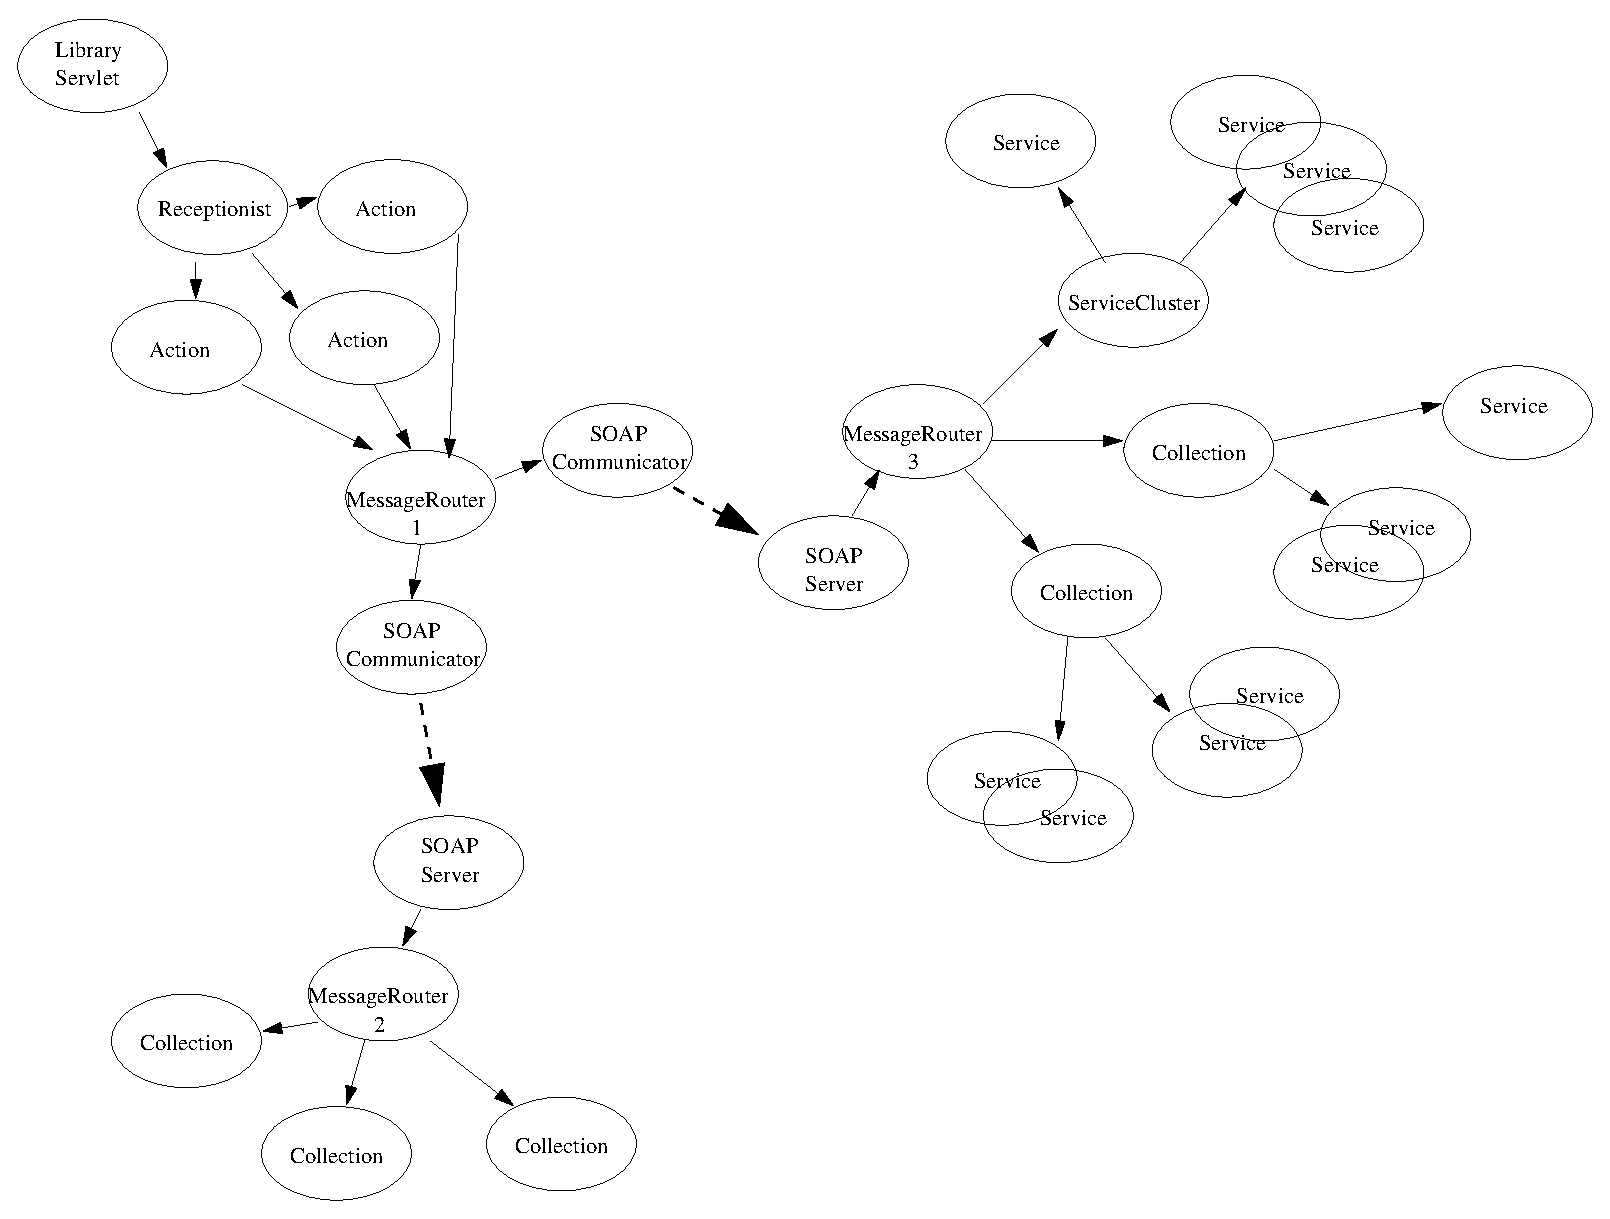
\includegraphics[width=4in]{remote} %5.8
  \caption{A distributed digital library configuration running over several servers}
  \label{fig:remote}
\end{figure}

We have used Apache Axis SOAP implementation. This is run as a servlet in Tomcat. Axis is set up during installation of Greenstone. For more details about SOAP in Greenstone, see Appendix~\ref{app:soap}. Debugging soap is described in Appendix~\ref{app:soap-debug}.

\subsection{Serving a site using soap}

A web service for localsite comes with \gs. However, it is not deployed by default. To deploy it, run run \gst{ant deploy-localsite}. If you want to set up web services for other sites, run \gst{ant soap-deploy-site}. This will prompt you for the sitename (its directory name), and a siteuri - a unique identifier for the web service. Tomcat needs to be running for this to work, and you need to have installed the \gs source code.

The ant target deploys the service for the site specified. A resource file (\gst{<sitename>.wsdd}) is created which is used to specify the service. It can be found in \gst{\$GSDL3HOME/resources/soap}, and is generated from \gst{site.wsdd.template}.

The address of the new SOAP service will be tomcatserver-address/greenstone3/services/sitename, for example, www.greenstone.org/greenstone3/services/localsite.

\subsection{Connecting to a site web service}

There are two ways to use a remote site. First, if you have a local site running, then the site can also connect to other remote sites. In the siteConfig.xml file, you need to add a site element into the siteList element.

For example, to get siteA to talk to siteB, you need to deploy a SOAP server on siteB, then add a \gst{<site>} element to the \gst{<siteList>} of siteA's \gst{siteConfig.xml} file (in \gst{\$GSDL3HOME/sites/siteA/siteConfig.xml}).

In the \gst{<siteList>} element, add the following (substituting the chosen site uri for siteBuri):

\begin{gsc}\begin{verbatim}
<site name="siteBuri"
  address="http://localhost:8080/greenstone3/services/siteBuri"
  type="soap"/>
\end{verbatim}\end{gsc}

(Note that localhost and 8080 should be changed to the values you entered when installing \gsiii. Localhost will only work for servers on the smae machine.).

If you have changed the siteConfig.xml file for a site that is running, it will need to be reconfigured. Either restart Tomcat, or reconfigure through a URL:
e.g. \gst{http://localhost:8080/greenstone3/library?a=s\&sa=c}.
Several sites can be connected to in this manner.

The second option is if you have a receptionist set up on a machine where you have no site, and you only want to connect to a single remote site. Instead of using site\_name in the servlet initialisation parameters (in \$GSDL3HOME/WEB-INF/web.xml), you can specify remote\_site\_name, remote\_site\_type and remote\_site\_address. A communicator object will be set up instead of a MessageRouter and the receptionist will talk to the communicator.

\appendix

\newpage
\section{Using \gsiii\  from CVS}\label{app:cvs}

\gsiii\  is also available via CVS. You can download the latest version of the code. This is not guaranteed to be stable, in fact it is likely to be unstable. The advantage of using CVS is that you can update the code and get the latest fixes. 

Note that you will need the Java 2 SDK, version 1.4.0 or higher, and Ant (Apache's Java based build tool, http://ant.apache.org) installed.

To check out the \gs\  code, use:

\begin{quote}\begin{gsc}\begin{verbatim}
cvs -d :pserver:cvs\_anon@cvs.scms.waikato.ac.nz:2402/usr/local/
           global-cvs/gsdl-src co -P greenstone3
\end{verbatim}\end{gsc}\end{quote}

If you need it, the password for anonymous CVS access is \gst{anonymous}. Note that some older versions of CVS have trouble accessing this repository due to the port number being present. We are using version 1.11.1p1. 

Greenstone is built and installed using Ant (Apache's Java based build tool, 
http://ant.apache.org). You will need a Java Development 
Environment (1.4 or higher), and Ant installed to use Greenstone. You can download Ant from \\\gst{http://ant.apache.org/bindownload.cgi}. Make sure that the environment variables JAVA\_HOME and ANT\_HOME are set.

In the \gst{greenstone3} directory, you can run \gst{'ant'} which will give you a help message.
Running \gst{'ant -projecthelp'} gives a list of the targets that you can run --- these
do various things like compile the source code, startup the server etc.

The \gst{README.txt} file has up-to-date instructions for installing from CVS. Briefly, for a first time install, run \gst{'ant prepare install'}.

The file \gst{build.properties} contains various parameters that can be set by the user. Please check these settings before running the installation process. The install process will ask you if you accept the properties before starting.
For a  non-interactive version of the install, run
\gst{'ant -Dproperties.accepted=yes install'}

To log the output in build.log, run
\gst{'ant -Dproperties.accepted=yes -logfile build.log install'}

Compilation includes Java and C/C++. On Windows, you will need to have Visual Studio or equivalent installed. Please check the \gst{compile.windows.c++.setup} property in build.properties --- make sure it is set to the setup script of Visual Studio.

Note: \gst{gs3-setup} sets the environment variables \gst{GSDL3HOME, GSDL3SRCHOME, CLASSPATH, PATH, JAVA\_HOME} and needs to be done in a shell before doing collection building etc. 

To run the library, use the \gst{gs3-server.sh/bat} shell scripts.

\newpage
\section{Tomcat}\label{app:tomcat}

Tomcat is a servlet container, and \gsiii\  runs as a servlet inside it. 

The file \gst{\$GSDL3SRCHOME/packages/tomcat/conf/server.xml} is the Tomcat configuration file. A context for \gsiii\  is given by the file\\ \gst{\$GSDL3SRCHOME/packages/tomcat/conf/Catalina/localhost/greenstone3.xml}. This tells Tomcat where to find the web.xml file, and what URL (\gst{/greenstone3}) to give it. Anything inside the context directory is accessible via Tomcat\footnote{can we use .htaccess files to restrict access??}. For example, the index.html file that lives in \gst{\$GSDL3HOME} can be accessed through the URL \gst{localhost:8080/greenstone3/index.html}. The gs2mgdemo collection's images can be accessed through \\
\gst{localhost:8080/greenstone3/sites/localsite/collect/gs2mgdemo/images/}.


Greenstone sets up Tomcat to run on port 8080 by default. To change this, you can edit the tomcat.port property in build.properties. If you do this before installing Greenstone, then running 'ant install' will use the new port number. If you want to change it later on, shutdown tomcat, run 'ant configure', then when you restart tomcat it will use the new port.

Note: Tomcat must be shutdown and restarted any time you make changes in the following for those changes to take effect:
\begin{bulletedlist}
\begin{gsc}
\item \$GSDL3HOME/WEB-INF/web.xml
\item \$GSDL3SRCHOME/packages/tomcat/conf/server.xml
\end{gsc}
\item any classes or jar files used by the servlets
\end{bulletedlist}

On startup, the servlet loads in its collections and services. If the site or collection configuration files are changed, these changes will not take effect until the site/collection is reloaded. This can be done through the reconfiguration messages (see Section~\ref{sec:runtime-config}), or by restarting Tomcat.

We have disabled following symlinks for the greenstone servlet. To enable it, edit \gst{\$GSDL3SRCHOME/packages/tomcat/conf/Catalina/localhost/greenstone3.xml} and set 'allowLinking' to true. 

By default, Tomcat allows directory listings. To disable this, change the 'listings' parameter to false in the default servlet definition, in Tomcat's web.xml file (\gst{\$GSDL3SRCHOME/packages/tomcat/conf/web.xml}):

We have set the greenstone context to be reloadable. This means that if a class or resource file in web/WEB-INF/lib or web/WEB-INF/classes changes, the servlet will be reloaded. This is useful for development, but should be turned off for production mode (set the 'reloadable' attribute to false).

Tomcat uses a Manager to handle HTTP session information. This may be stored between restarts if possible. To use a persistent session handling manager, uncomment the \gst{<Manager>} element in \\
\gst{\$GSDL3SRCHOME/packages/tomcat/conf/server.xml}. For the default manager, session information is stored in the work directory:\\
\gst{\$GSDL3SRCHOME/packages/tomcat/work/Catalina/localhost/greenstone3/SESSIONS.ser}. Delete this file to clear the cached session info. Note that Tomcat needs to be shutdown to delete this file.

\subsection{Proxying Tomcat with apache}

Instead of incorporating servlet support into your existing web server, an easy alternative is to proxy Tomcat. The \gst{http://www.greenstone.org/greenstone3} site uses apache to proxy Tomcat. ProxyPass and ProxyPassReverse directives need to be added to the Virtualhost description for the www.greenstone.org server.

\begin{quote}\begin{gsc}
<VirtualHost xx.xx.xx.xx>\\
ServerName www.greenstone.org\\
...\\
ProxyPass /greenstone3 http://puka.cs.waikato.ac.nz:8080/greenstone3\\
ProxyPassReverse /greenstone3 http://puka.cs.waikato.ac.nz:8080/greenstone3\\
</VirtualHost>\\
\end{gsc}\end{quote}

In our example, the \gsiii\  servlet can be accessed at \\
\gst{http://www.greenstone.org/greenstone3/library}, instead of at \\
\gst{http://puka.cs.waikato.ac.nz:8080/greenstone3/library}, which is not publically accessible.

\subsection{Running Tomcat behind a proxy}

Almost everything works fine when Tomcat is running behind a proxy. The only time this causes trouble is if the servlet itself needs to make external HTTP connections. We do this in the infomine demo collection for example. One of the service classes sends HTTP requests to the infomine database at riverside. Since this is going through the proxy, a username and password is needed. It is not sufficient to prompt the user for a password because they are unlikely to have a password for the particular proxy that Tomcat is using. What we have done at present is to put a proxy element in the siteConfig.xml file. Here you have to enter a suitable username and password for the proxy server. Unfortunately these are entered in plain text. And the file is viewable via the servlet. So we need a better solution.

\newpage
\section{SOAP}\label{app:soap}

Greenstone uses the Apache Axis SOAP implementation for distributed communications. Axis runs as a servlet inside Tomcat, and SOAP web services can be deployed by this Axis servlet. The Greenstone installation process sets up Axis for Tomcat, but does not deploy any services. 

To deploy the SOAP service for localsite, run \gst{ant deploy-localsite}.

To deploy a SOAP service for other sites, run \gst{ant soap-deploy-site}

This will prompt you for the sitename (the site's directory name), and a unique URI for the site. It creates a new SOAPServer class for the site \\(\gst{\$GSDL3SRCHOME/src/java/org/greenstone/gsdl3/SOAPServer<sitename>.java}), creates a resource file for deployment (\gst{\$GSDL3SRCHOME/resources/soap/<sitename>.wsdd}), and then tries to deploy the service.

Information about deployed services is maintained between Tomcat sessions---you only need to deploy something once. To undeploy a site, use \gst{ant soap-undeploy-site}.

The axis services can be accessed at \gst{localhost:8080/greenstone3/index.jsp}.

\subsection{Debugging SOAP}\label{app:soap-debug}

If you need to debug the SOAP stuff for some reason, or just want to look at the SOAP messages that are being passed back and forth, you can use the TCP monitor. This intercepts messages coming in to one port, displays them, and passes them to another port.
To run it, type:

\begin{quote}\gst{java -cp \$GSDL3HOME/WEB-INF/lib/axis.jar \\
org.apache.axis.utils.tcpmon}
\end{quote}

The listen port is the port that you want the monitor to be listening on. It should 'act as' a Listener, with target hostname 127.0.0.1 (localhost), and target port the port that Tomcat is running on (8080). You need to modify the address used to talk to the SOAP service. For example, if you want to monitor traffic between the gateway site and the localsite SOAP server, you will need to edit gateway's siteConfig.xml file and change the port number (in the site element) to whatever you have chosen as the listen port.

For example, in the Admin panel of TCPMonitor the Target Hostname might be 127.0.0.1, and the Target Port \# 8080. Set the Listen Port \# to be a different port, such as 8070 and click Add. This produces a new tab panel where you can see the messages arriving at port 8070 before being forwarded to port 8080. You then need to set your test request from your SOAP application to arrive at port 8070 and you will see copies of the messages in the new tab panel.


\newpage
\section{Tidying up the formatting for imported \gsii\  collections}\label{app:gs2tidy}

\subsection{Format statements: \gsii\  vs \gsiii\ }\label{app:gs2format}
The following table shows the \gsii\  format elements, and their equivalents in \gsiii\ 
\begin{table}[h]
\caption{\gsiii\  equivalents of \gsii\  format statements}
{\footnotesize
\begin{tabular}{ll}
\hline
\bf \gsii\         & \bf \gsiii\  \\
\hline
\gst{[Text]} & \gst{<gsf:text/>} \\
\gst{[num]} & \gst{<gsf:metadata name='docnum'/>}\\
\gst{[link][/link]} & \gst{<gsf:link></gsf:link>} or \\
& \gst{<gsf:link type='document'></gsf:link>}\\
\gst{[srclink][/srclink]} & \gst{<gsf:link type='source'></gsf:link>}\\
\gst{[icon]} & \gst{<gsf:icon/>} or \\
& \gst{<gsf:icon type='document'/>}\\
\gst{[srcicon]} & \gst{<gsf:icon type='source'/>}\\
\gst{[Title]} (metadata) & \gst{<gsf:metadata name='Title'/>} or \\
& \gst{<gsf:metadata name='Title' select='current'/>}\\
\gst{[parent:Title]} & \gst{<gsf:metadata name='Title' select='parent' />}\\
\gst{[parent(All):Title]} & \gst{<gsf:metadata name='Title' select='ancestors'/>}\\
\gst{[parent(Top):Title]} & \gst{<gsf:metadata name='Title' select='root' />}\\
\gst{[parent(All': '):Title]} & \gst{<gsf:metadata name='Title' select='ancestors'}\\ 
& \gst{  separator=': ' />}\\
\gst{[sibling:dc.Title]} & \gst{<gsf:metadata name='dc.Title' pos='first'} \\
\gst{[sibling(All': '):Title]} & \gst{<gsf:metadata name='Title'} \\
& \gst{  separator=': ' />}\\
\gst{\{Or\}\{[dc.Title],}  & \gst{<gsf:choose-metadata>}\\
\gst{  [dls.Title], [Title]\}}& \gst{  <gsf:metadata name='dc.Title'/>}\\
& \gst{  <gsf:metadata name='dls.Title'/>}\\
& \gst{  <gsf:metadata name='Title'/>}\\
& \gst{</gsf:choose-metadata>}\\
\gst{\{If\}\{[parent:Title],} & \gst{<gsf:choose-metadata>}\\
\gst{  [parent:Title], [Title]\}}& \gst{  <gsf:metadata name='Title' select='parent'/>}\\
& \gst{  <gsf:metadata name='Title'/>}\\
& \gst{</gsf:choose-metadata>}\\
\gst{\{If\}\{[Subject],} & \gst{<gsf:switch>}\\
\gst{  <td>[Subject]</td>\}}& \gst{  <gsf:metadata name='Subject'/>}\\
& \gst{  <gsf:when test='exists'>} \\
& \gst{     <td><gsf:metadata name='Subject'/></td>}\\
& \gst{  </gsf:when></gsf:switch>}\\
\hline
\end{tabular}}
\end{table}
\subsection{Cleaning up macros}\label{app:gs2replace}

Here we show some of the replace items that have been used for \gsii\  collections.

Getting rid of silly backslashes:
\begin{gsc}\begin{verbatim}
<replace scope='text' macro="\\?\\\(" text="\("/>
\end{verbatim}\end{gsc}

Macro resolving using resource bundles and metadata:
\begin{gsc}\begin{verbatim}
<replace scope='metadata' macro="_magazines_" bundle="NZDLMacros" 
   key="Magazines"/>
<replace scope='all' macro='_thisOID_' metadata='archivedir'/>
<replace macro="_httpcollimg_" 
   text="sites/localsite/collect/folktale/index/assoc"/>
\end{verbatim}\end{gsc}

Fixing up broken external links:
\begin{gsc}\begin{verbatim}
<replace macro="_httpextlink_&amp;rl=1&amp;href=" 
   text="?a=d&amp;c=folktale&amp;s0.ext=1&amp;d="/>
<replace macro="_httpextlink_&amp;rl=0&amp;href=" 
   text="?a=p&amp;sa=html&amp;c=folktale&amp;url="/>
\end{verbatim}\end{gsc}

These two examples show how to deal with \gsii's external link macros. The first one is for a 'relative' external link. In this case, the links are like URL's but they actually refer to Greenstone internal documents. So the \gsiii\  link is to the document, but with parameter s0.ext signifying that the d argument will need translating before retrieving the content.
The second example is a truly external link. This is translated into a HTML type page action, where the URL is presented as a frame along with the collection header in a separate frame.

Sometimes we need to add in macros to be resolved in a second step:
\begin{gsc}\begin{verbatim}
<replace macro="_iconpdf_" scope="metadata" 
   text="&lt;img title='_texticonpdf_' src='interfaces/default/images/ipdf.gif'/&gt;"/>
<replace macro="_texticonpdf_" scope="metadata" bundle="interface_gs2" 
   key="texticonpdf"/>
\end{verbatim}\end{gsc}

\end{document}
